\documentclass[aspectratio=169]{beamer}
\usepackage{./tex_refs/tomcom}

\usefonttheme{serif}

\title{Railway track fault detection}
\author{Tamás DEMUS (XP4B9D)}
\date{26\textsuperscript{th} of June 2023}

\begin{document}

\begin{frame}
    \thispagestyle{empty}
    \begin{center}

        {\Large\textbf{Railway track fault detection}}

        \vspace*{0.5cm}

        Thesis presentation

        \vspace*{0.5cm}

        \begin{columns}[c]
            \begin{column}{0.45\textwidth}
                \centering
                {\small
                    Author:

                    \textbf{\textsc{Tamás Demus}}

                    XP4B9D
                }
            \end{column}
            \begin{column}{0.45\textwidth}
                \centering
                {\small
                    Supervisor:

                    \textsc{Dr. András Lukács}

                    Department of Computer Science
                }
            \end{column}
        \end{columns}

        \vspace*{\fill}

        \begin{columns}[c]
            \begin{column}{0.45\textwidth}
                \begin{figure}[H]
                    \raggedleft
                    
\includegraphics[width=0.25\textwidth]{./tex_images/elte_logo.png}
                \end{figure}
            \end{column}
            \begin{column}{0.45\textwidth}
                {\footnotesize\textsc{Eötvös Lóránd University}}

                {\footnotesize\textsc{Faculty of Science}}

                {\footnotesize\textsc{AI Research Group}}
            \end{column}
        \end{columns}

        \vspace*{0.5cm}

        {\small Budapest, 2023}
    \end{center}
\end{frame}

\begin{frame}{Table of Contents}
    \tableofcontents
\end{frame}

\section{Problem statement}
\begin{frame}{Railway track data}
    \begin{columns}[c]
        \begin{column}{0.25\textwidth}
            \begin{figure}
                \raggedright
                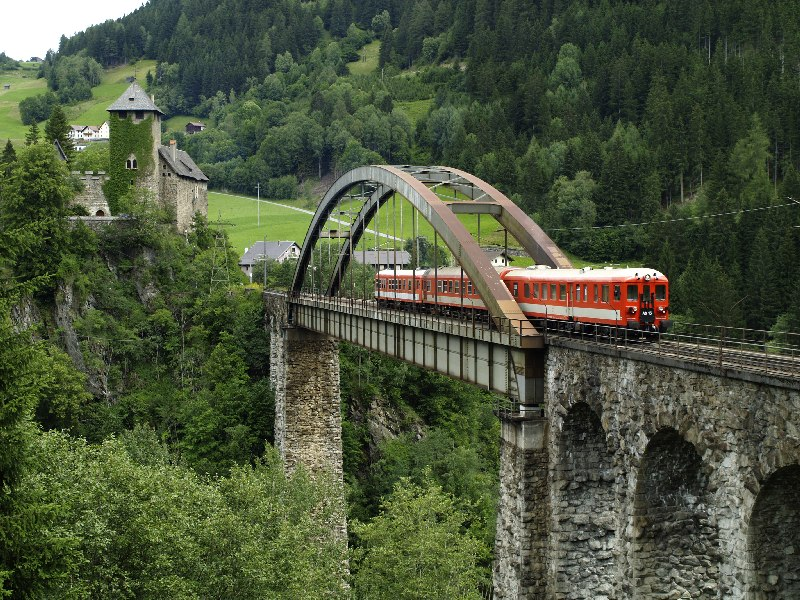
\includegraphics[width=\columnwidth]{./tex_images/sds.jpg}
                \caption*{SDS inspection vehicle}
                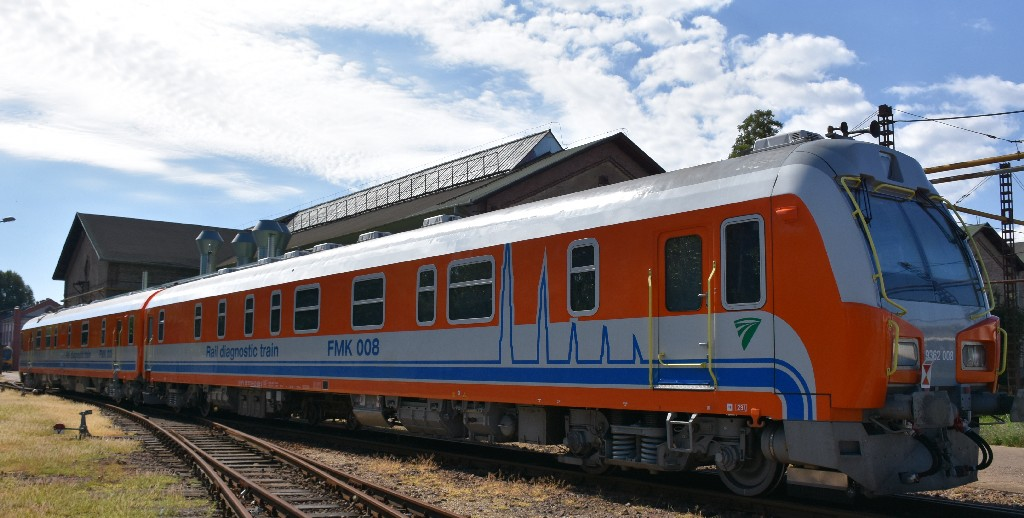
\includegraphics[width=\columnwidth]{./tex_images/FMK008.jpg}
                \caption*{FMK-008 vehicle}
            \end{figure}
        \end{column}
        \begin{column}{0.7\textwidth}
            MÁV Central Rail and Track Inspection Ltd.
            \begin{itemize}
                \item Performs rail and track inspection
                \item 2 inspection vehicles
                \item Equipped with camera systems
                \item Close view of the rail
                \item Approx. 3.5-minute sample video provided
                \item Additional hundred hours of footage
            \end{itemize}
        \end{column}
    \end{columns}
\end{frame}

\begin{frame}{Examples}
    \begin{figure}
        \centering
        \begin{subfigure}{0.3\textwidth}
            \centering
            \includegraphics[width=\textwidth]{./data/sd1_sample/normal/img_00006.jpg}
            \caption*{Normal rail}
        \end{subfigure}
        \begin{subfigure}{0.3\textwidth}
            \centering
            \includegraphics[width=\textwidth]{./data/sd1_sample/normal/img_00723.jpg}
            \caption*{Normal rail}
        \end{subfigure}
        \begin{subfigure}{0.3\textwidth}
            \centering
            \includegraphics[width=\textwidth]{./data/sd1_sample/normal/img_04857.jpg}
            \caption*{Normal rail}
        \end{subfigure}
        \begin{subfigure}{0.3\textwidth}
            \centering
            \includegraphics[width=\textwidth]{./data/sd1_sample/grass/img_05649.jpg}
            \caption*{Rails covered with grass}
        \end{subfigure}
        \begin{subfigure}{0.3\textwidth}
            \centering
            \includegraphics[width=\textwidth]{./data/sd1_sample/double_rail/img_05676.jpg}
            \caption*{Double rails}
        \end{subfigure}
    \end{figure}
\end{frame}

\section{Model description}
\begin{frame}{Model selection}
    \begin{figure}[t]
        \centering
        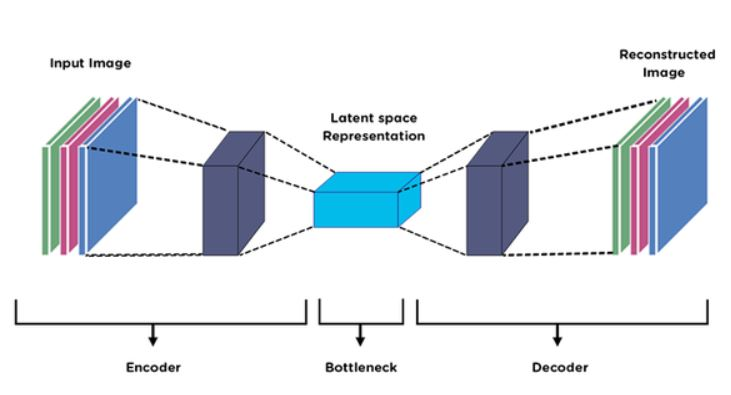
\includegraphics[width=0.45\textwidth,trim={0 0 0 1cm},clip]{./tex_images/autoencoder.jpeg}
        \caption*{General structure of Autoencoders}
    \end{figure}
    \begin{columns}[T]
        \begin{column}{0.25\textwidth}
            Encoders:
            \begin{itemize}
                \item VGG19 (BN)
                \item ResNet50
                \item EfficientNetV2L
            \end{itemize}
        \end{column}
        \begin{column}{0.25\textwidth}
            \centering
            Bottleneck

            Filter matching
        \end{column}
        \begin{column}{0.25\textwidth}
            Decoder:
            \begin{itemize}
                \item Inverse VGG19
            \end{itemize}
        \end{column}
    \end{columns}
\end{frame}

\begin{frame}[t]{Anomaly detection}
    \begin{columns}[T]
        \begin{column}{0.45\textwidth}
            Loss-based
        \end{column}
        \begin{column}{0.45\textwidth}
            Isolation Forest
        \end{column}
    \end{columns}
\end{frame}

\section{Results}
\begin{frame}[t]{Reconstructed images}
    \begin{columns}
        \begin{column}{0.2\textwidth}
            \centering
            VGG19
        \end{column}
        \begin{column}{0.75\textwidth}
            \begin{figure}
                \centering
                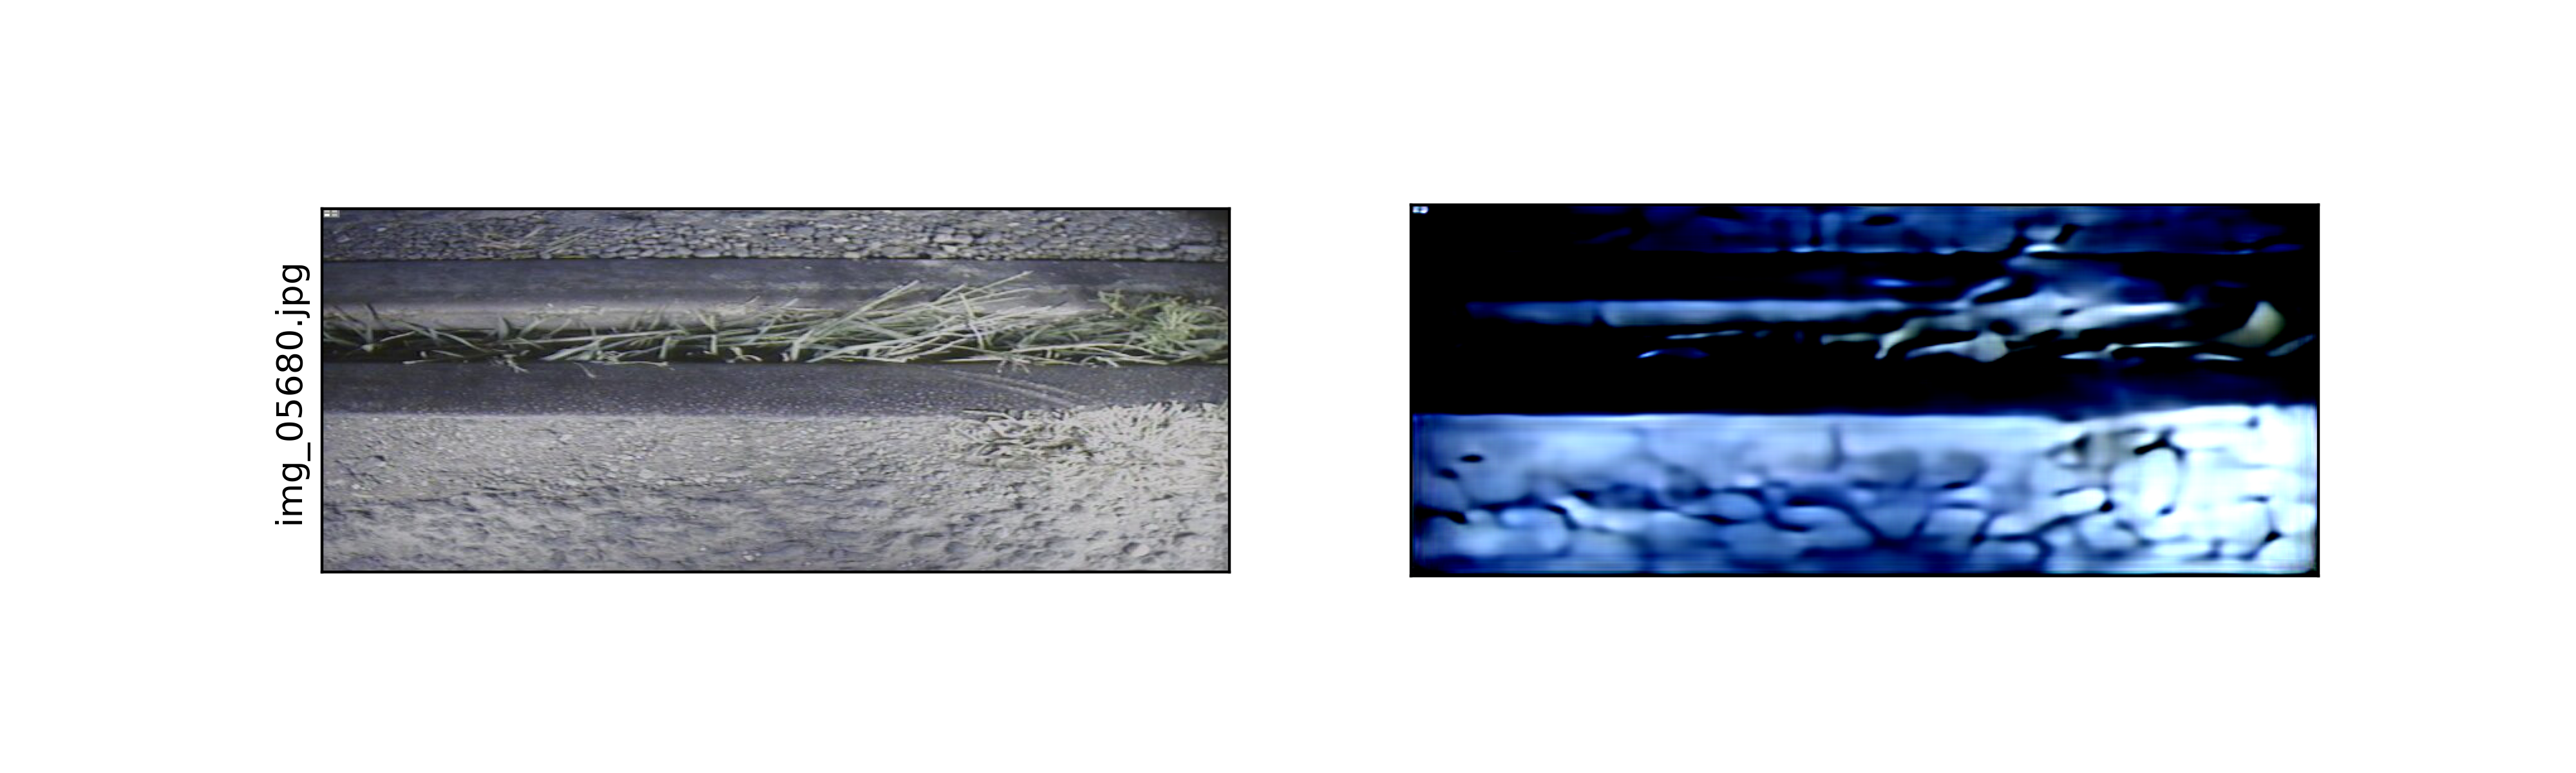
\includegraphics[width=\columnwidth,trim={0 1cm 0 1cm},clip]{./results/vgg19_vgg19/20230510_172958_predict_0.png}
            \end{figure}
        \end{column}
    \end{columns}
    \begin{columns}
        \begin{column}{0.2\textwidth}
            \centering
            VGG19 BN
        \end{column}
        \begin{column}{0.75\textwidth}
            \begin{figure}
                \centering
                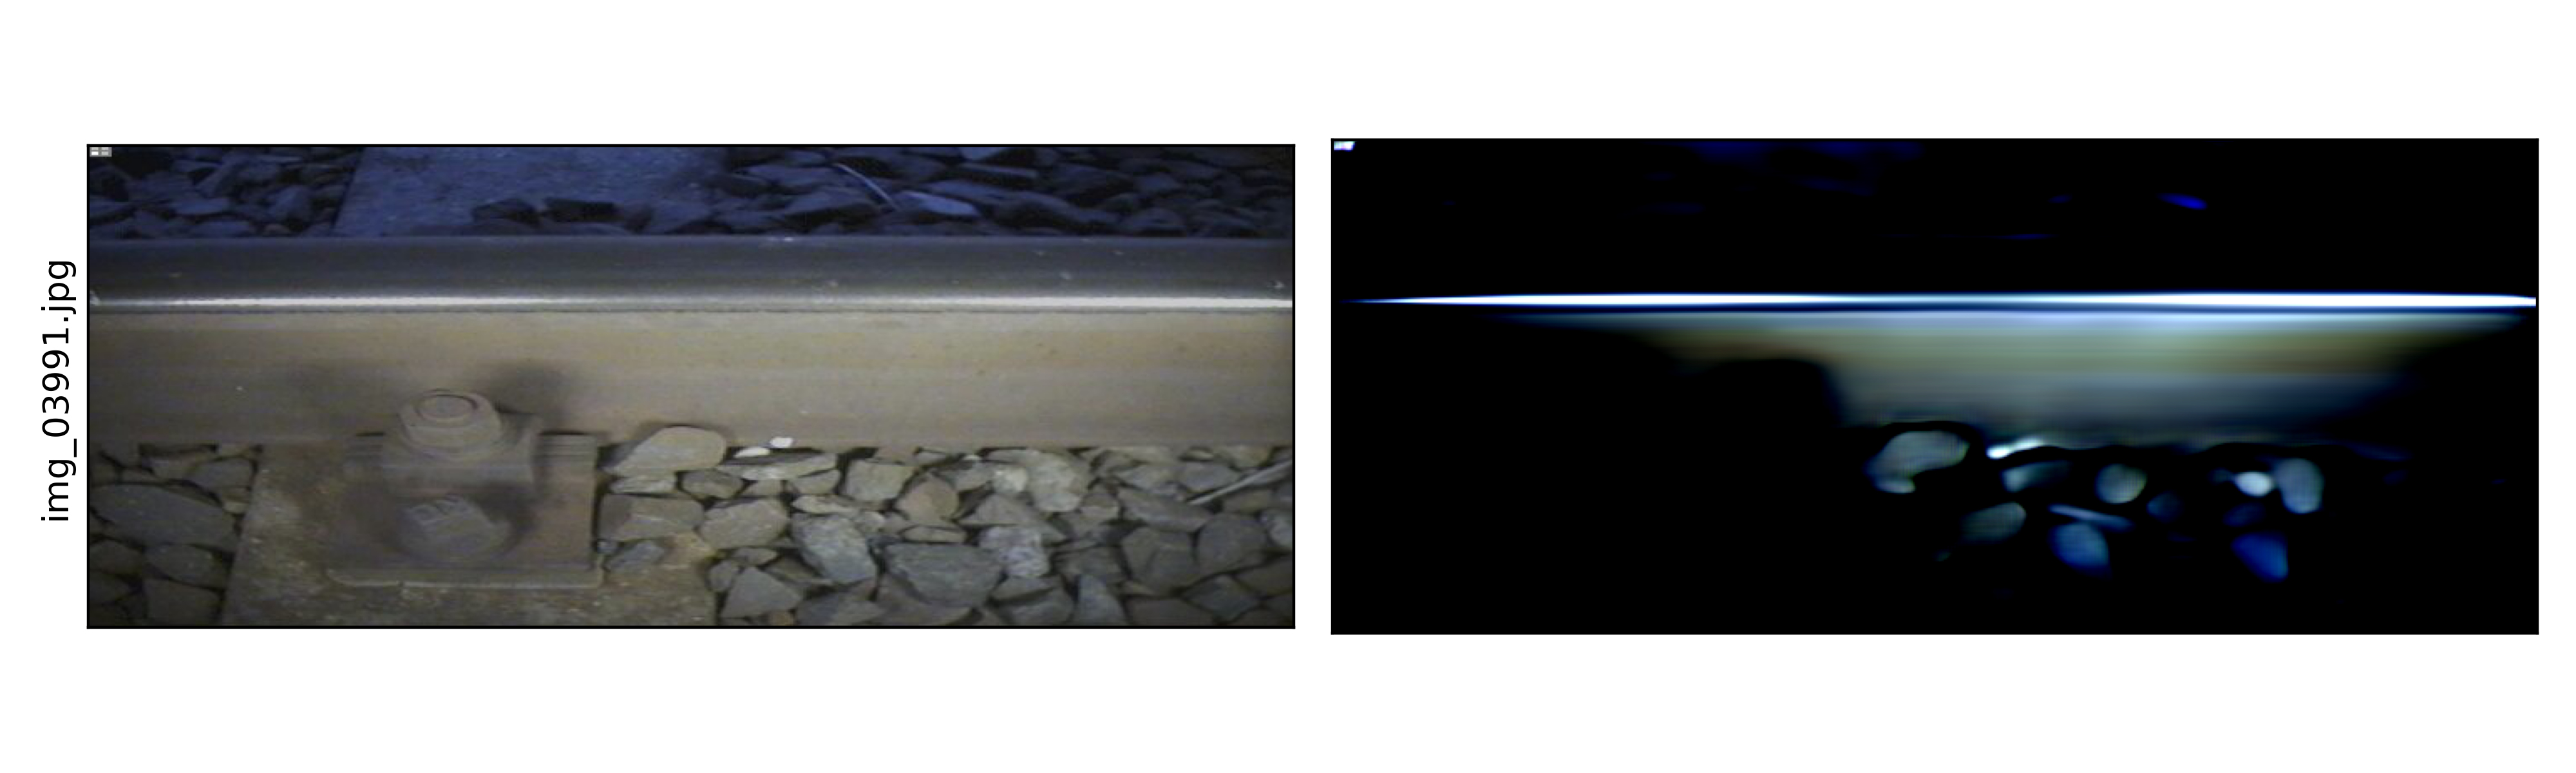
\includegraphics[width=\columnwidth,trim={0 1cm 0 1cm},clip]{./results/vgg19_bn_vgg19/20230525_045131_predict_0.png}
            \end{figure}
        \end{column}
    \end{columns}
\end{frame}

\begin{frame}[t]{Reconstructed images}
    \begin{columns}
        \begin{column}{0.2\textwidth}
            \centering
            ResNet50
        \end{column}
        \begin{column}{0.75\textwidth}
            \begin{figure}
                \centering
                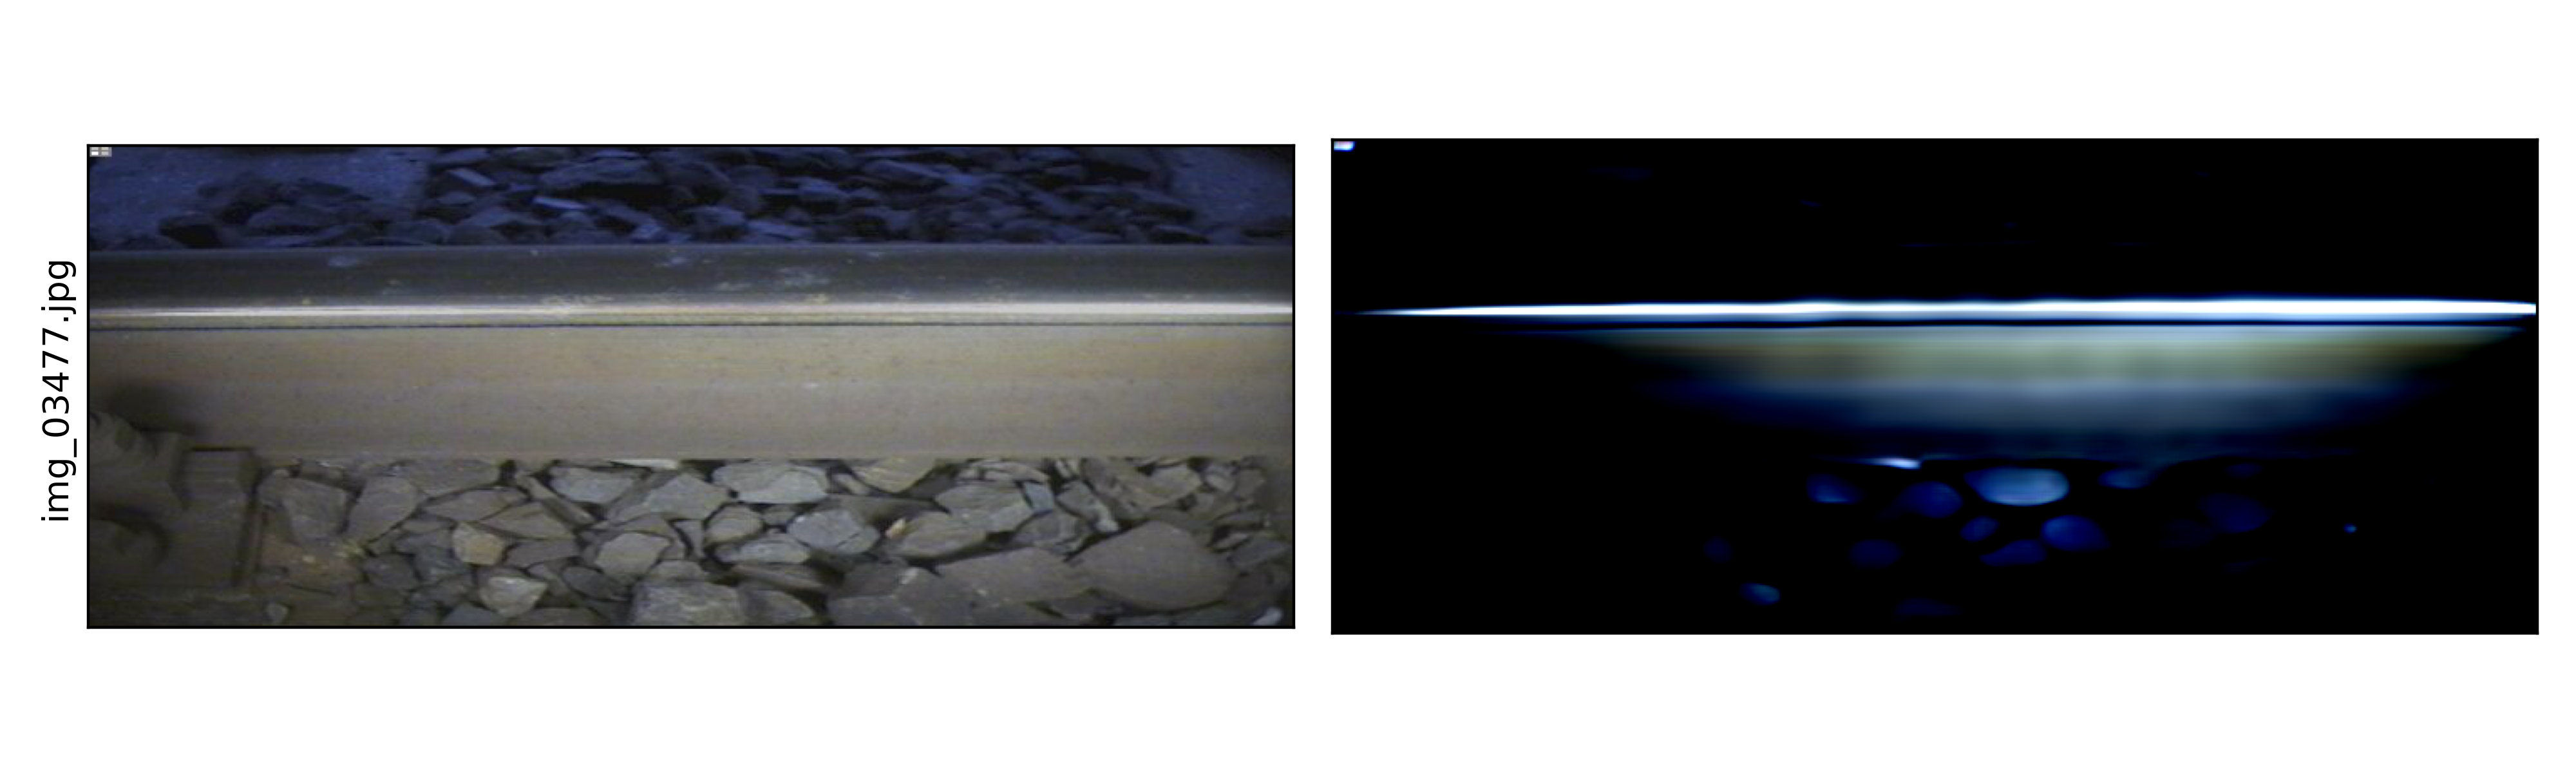
\includegraphics[width=\columnwidth,trim={0 1cm 0 1cm},clip]{./results/resnet50_vgg19/20230514_213740_predict_0.png}
            \end{figure}
        \end{column}
    \end{columns}
    \begin{columns}
        \begin{column}{0.2\textwidth}
            \centering
            EfficientNetV2L
        \end{column}
        \begin{column}{0.75\textwidth}
            \begin{figure}
                \centering
                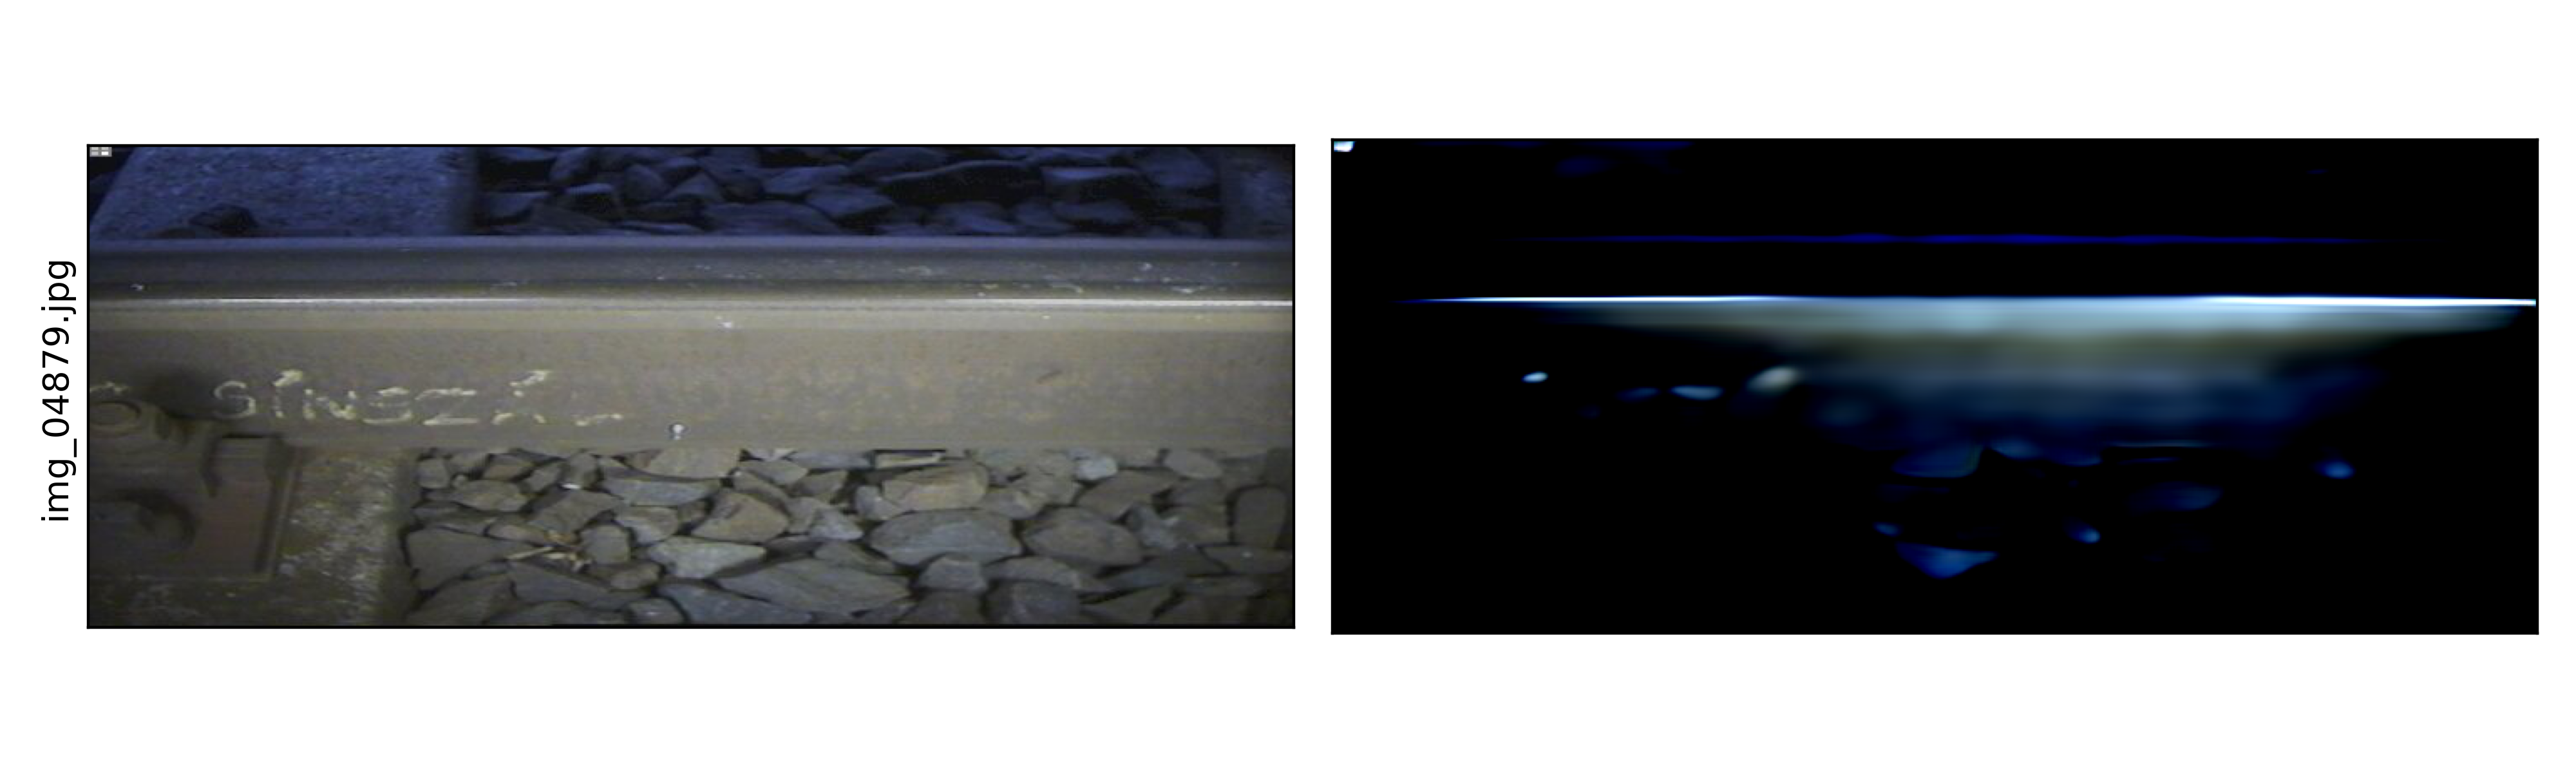
\includegraphics[width=\columnwidth,trim={0 1cm 0 1cm},clip]{./results/efficientnetv2l_vgg19/20230525_194238_predict_0.png}
            \end{figure}
        \end{column}
    \end{columns}
\end{frame}

\begin{frame}{Latent space visualization}
    \begin{columns}
        \begin{column}{0.45\textwidth}
            \begin{figure}
                \centering
                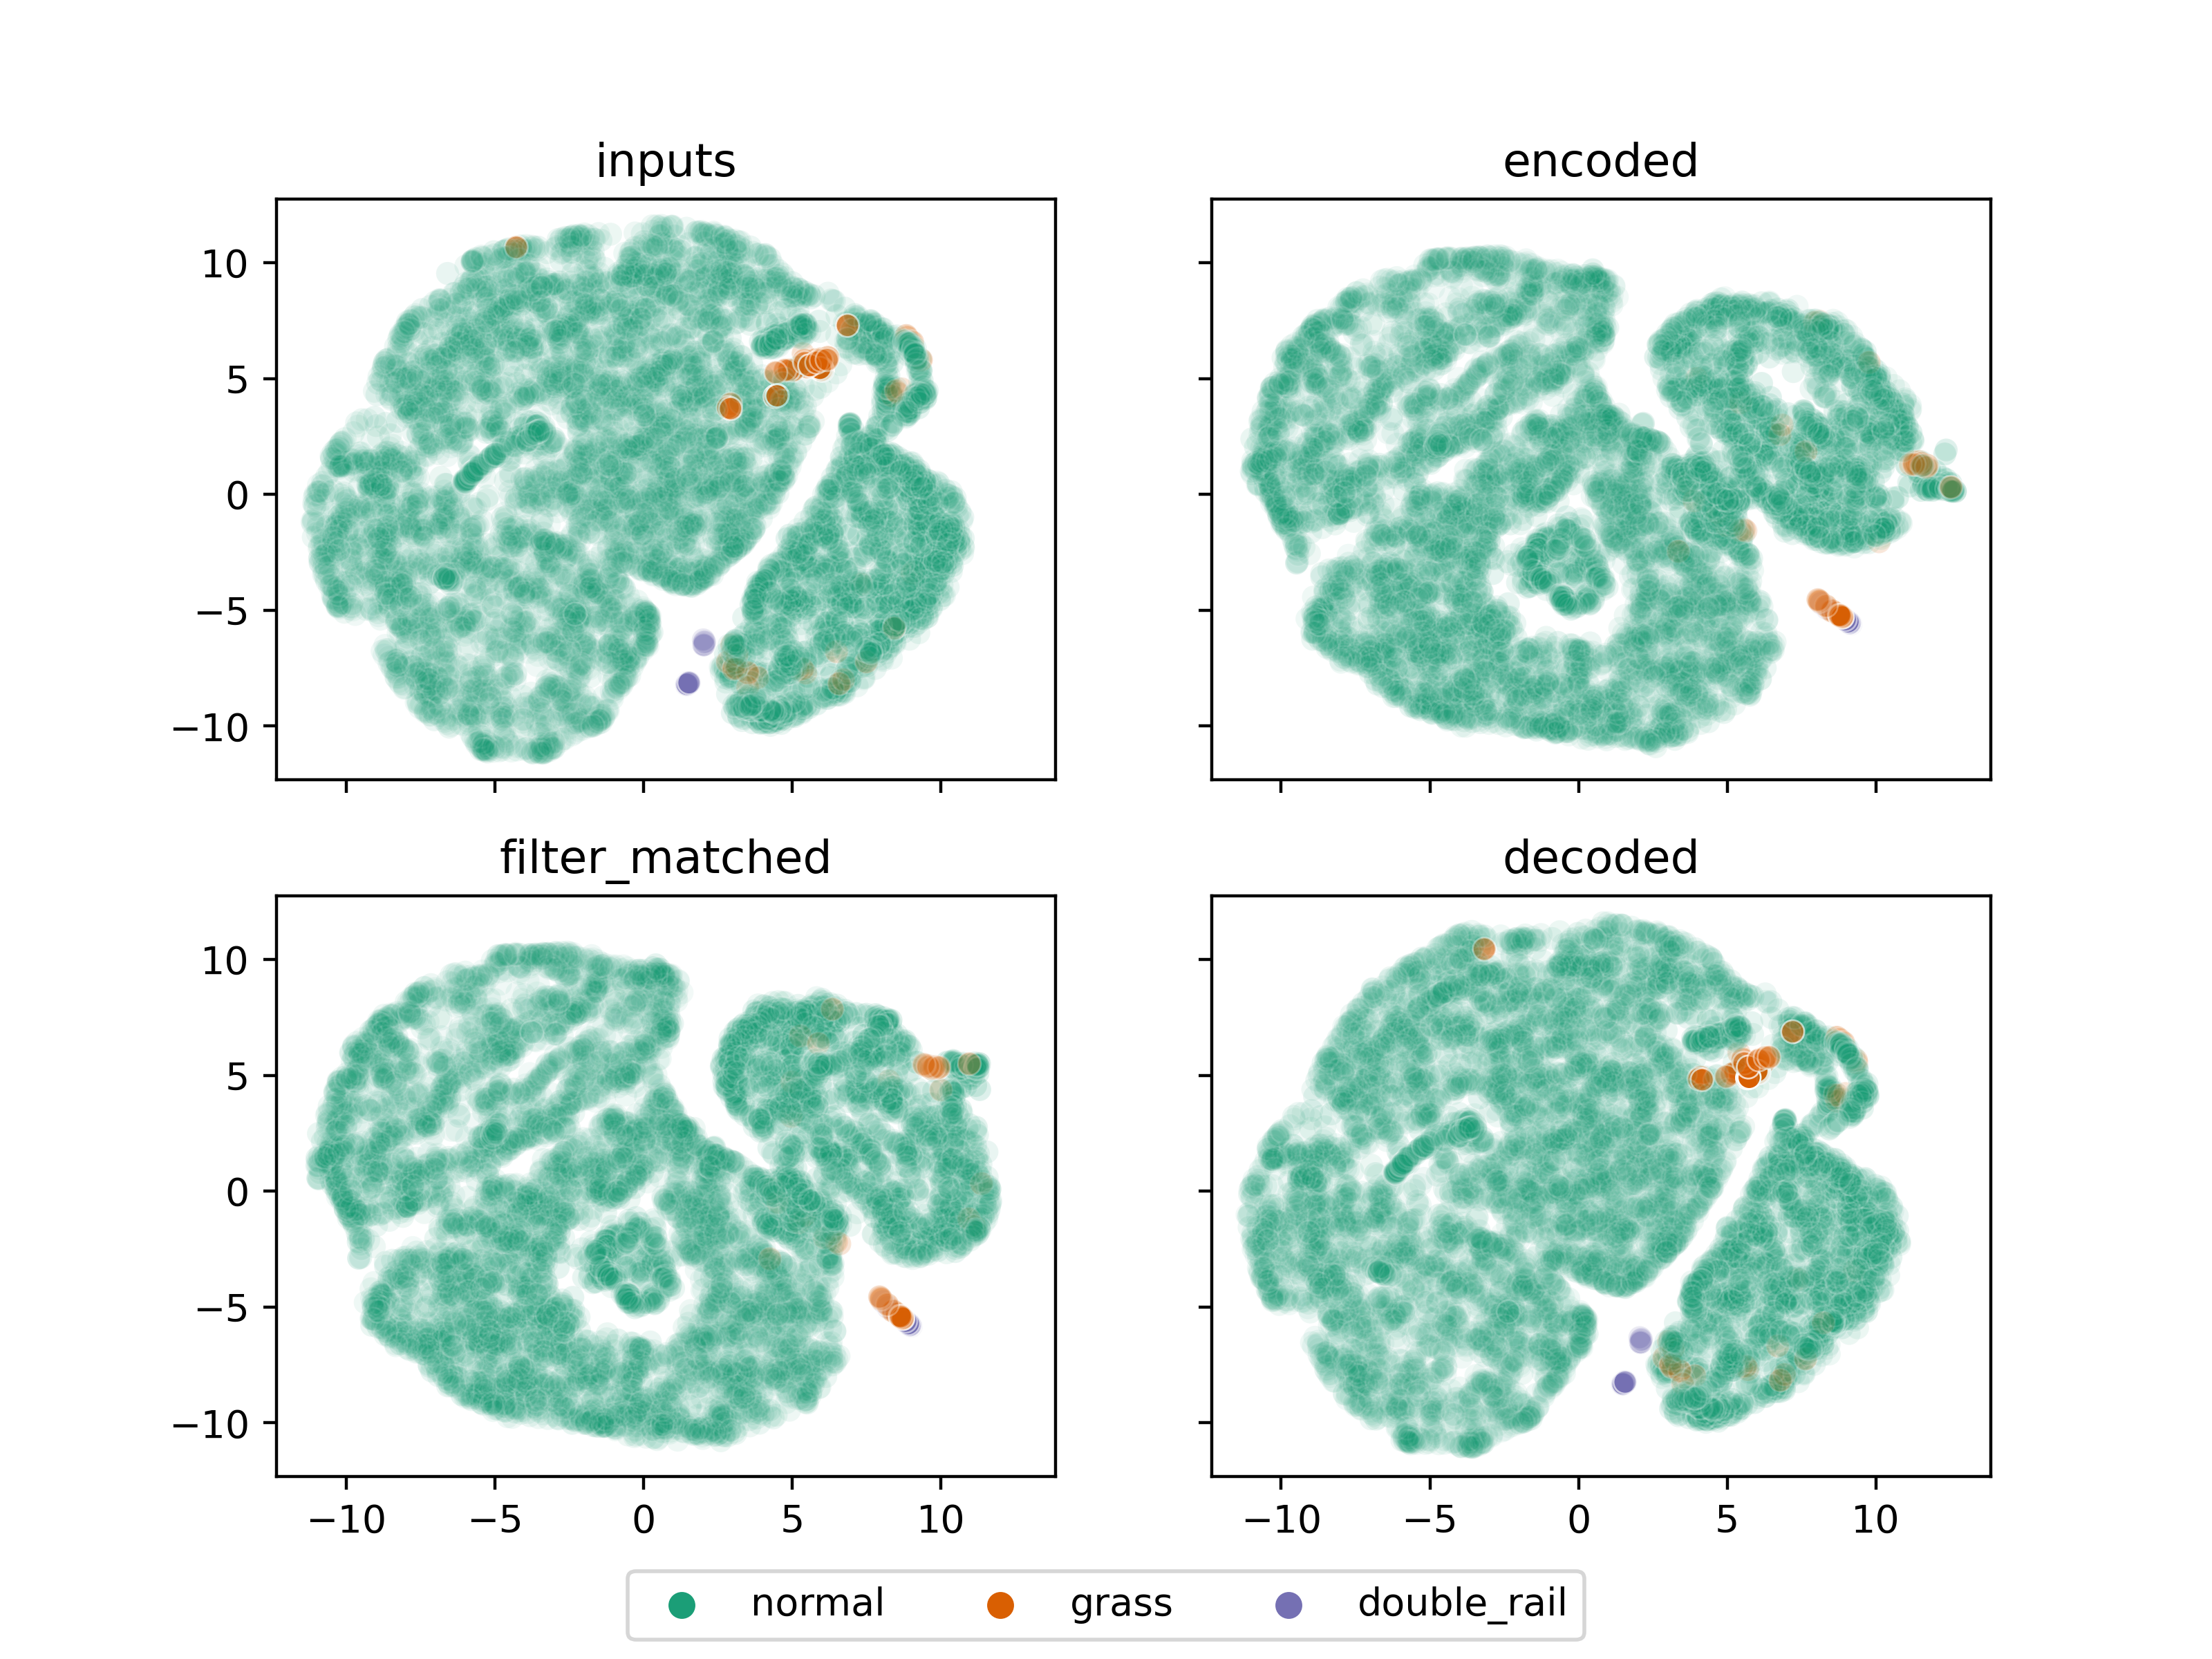
\includegraphics[width=\columnwidth,trim={0 0 0 1cm},clip]{./results/vgg19_vgg19/20230510_172958_feature_vectors_1.png}
                \caption*{VGG19}
            \end{figure}
        \end{column}
        \begin{column}{0.45\textwidth}
            \begin{figure}
                \centering
                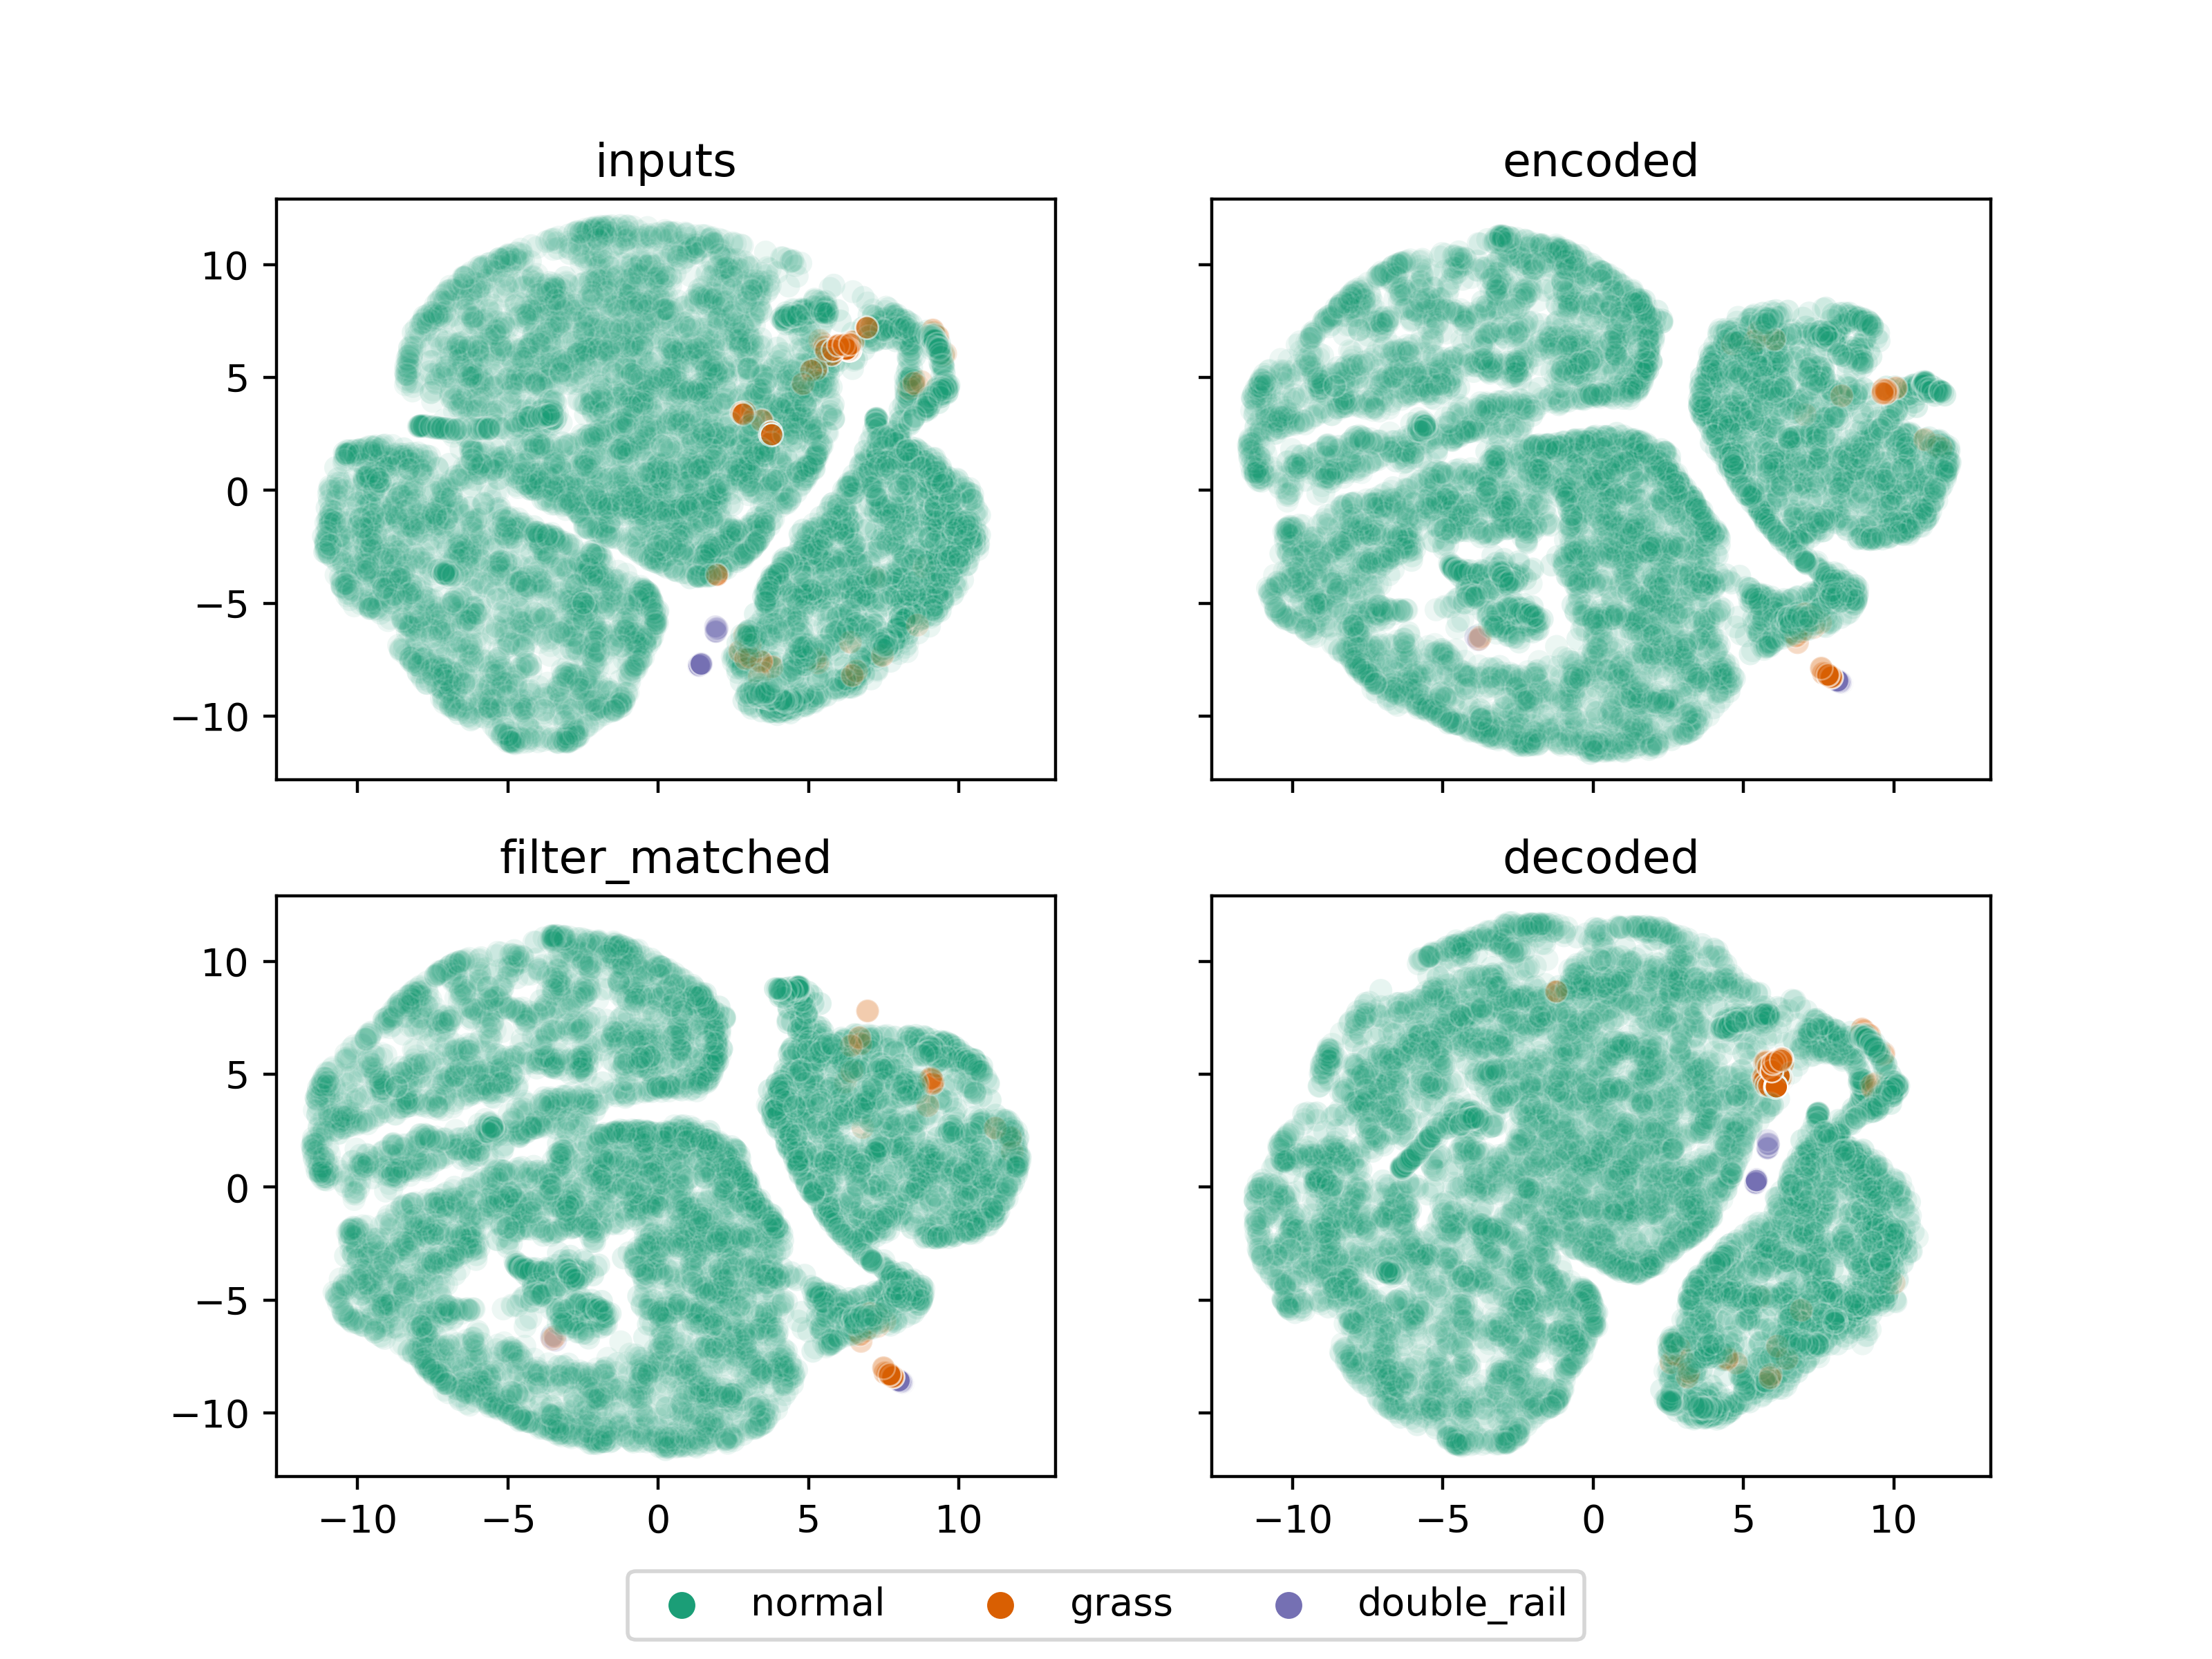
\includegraphics[width=\columnwidth,trim={0 0 0 1cm},clip]{./results/vgg19_bn_vgg19/20230525_045131_feature_vectors_1.png}
                \caption*{VGG19 BN}
            \end{figure}
        \end{column}
    \end{columns}
\end{frame}
\begin{frame}{Latent space visualization}
    \begin{columns}
        \begin{column}{0.45\textwidth}
            \begin{figure}
                \centering
                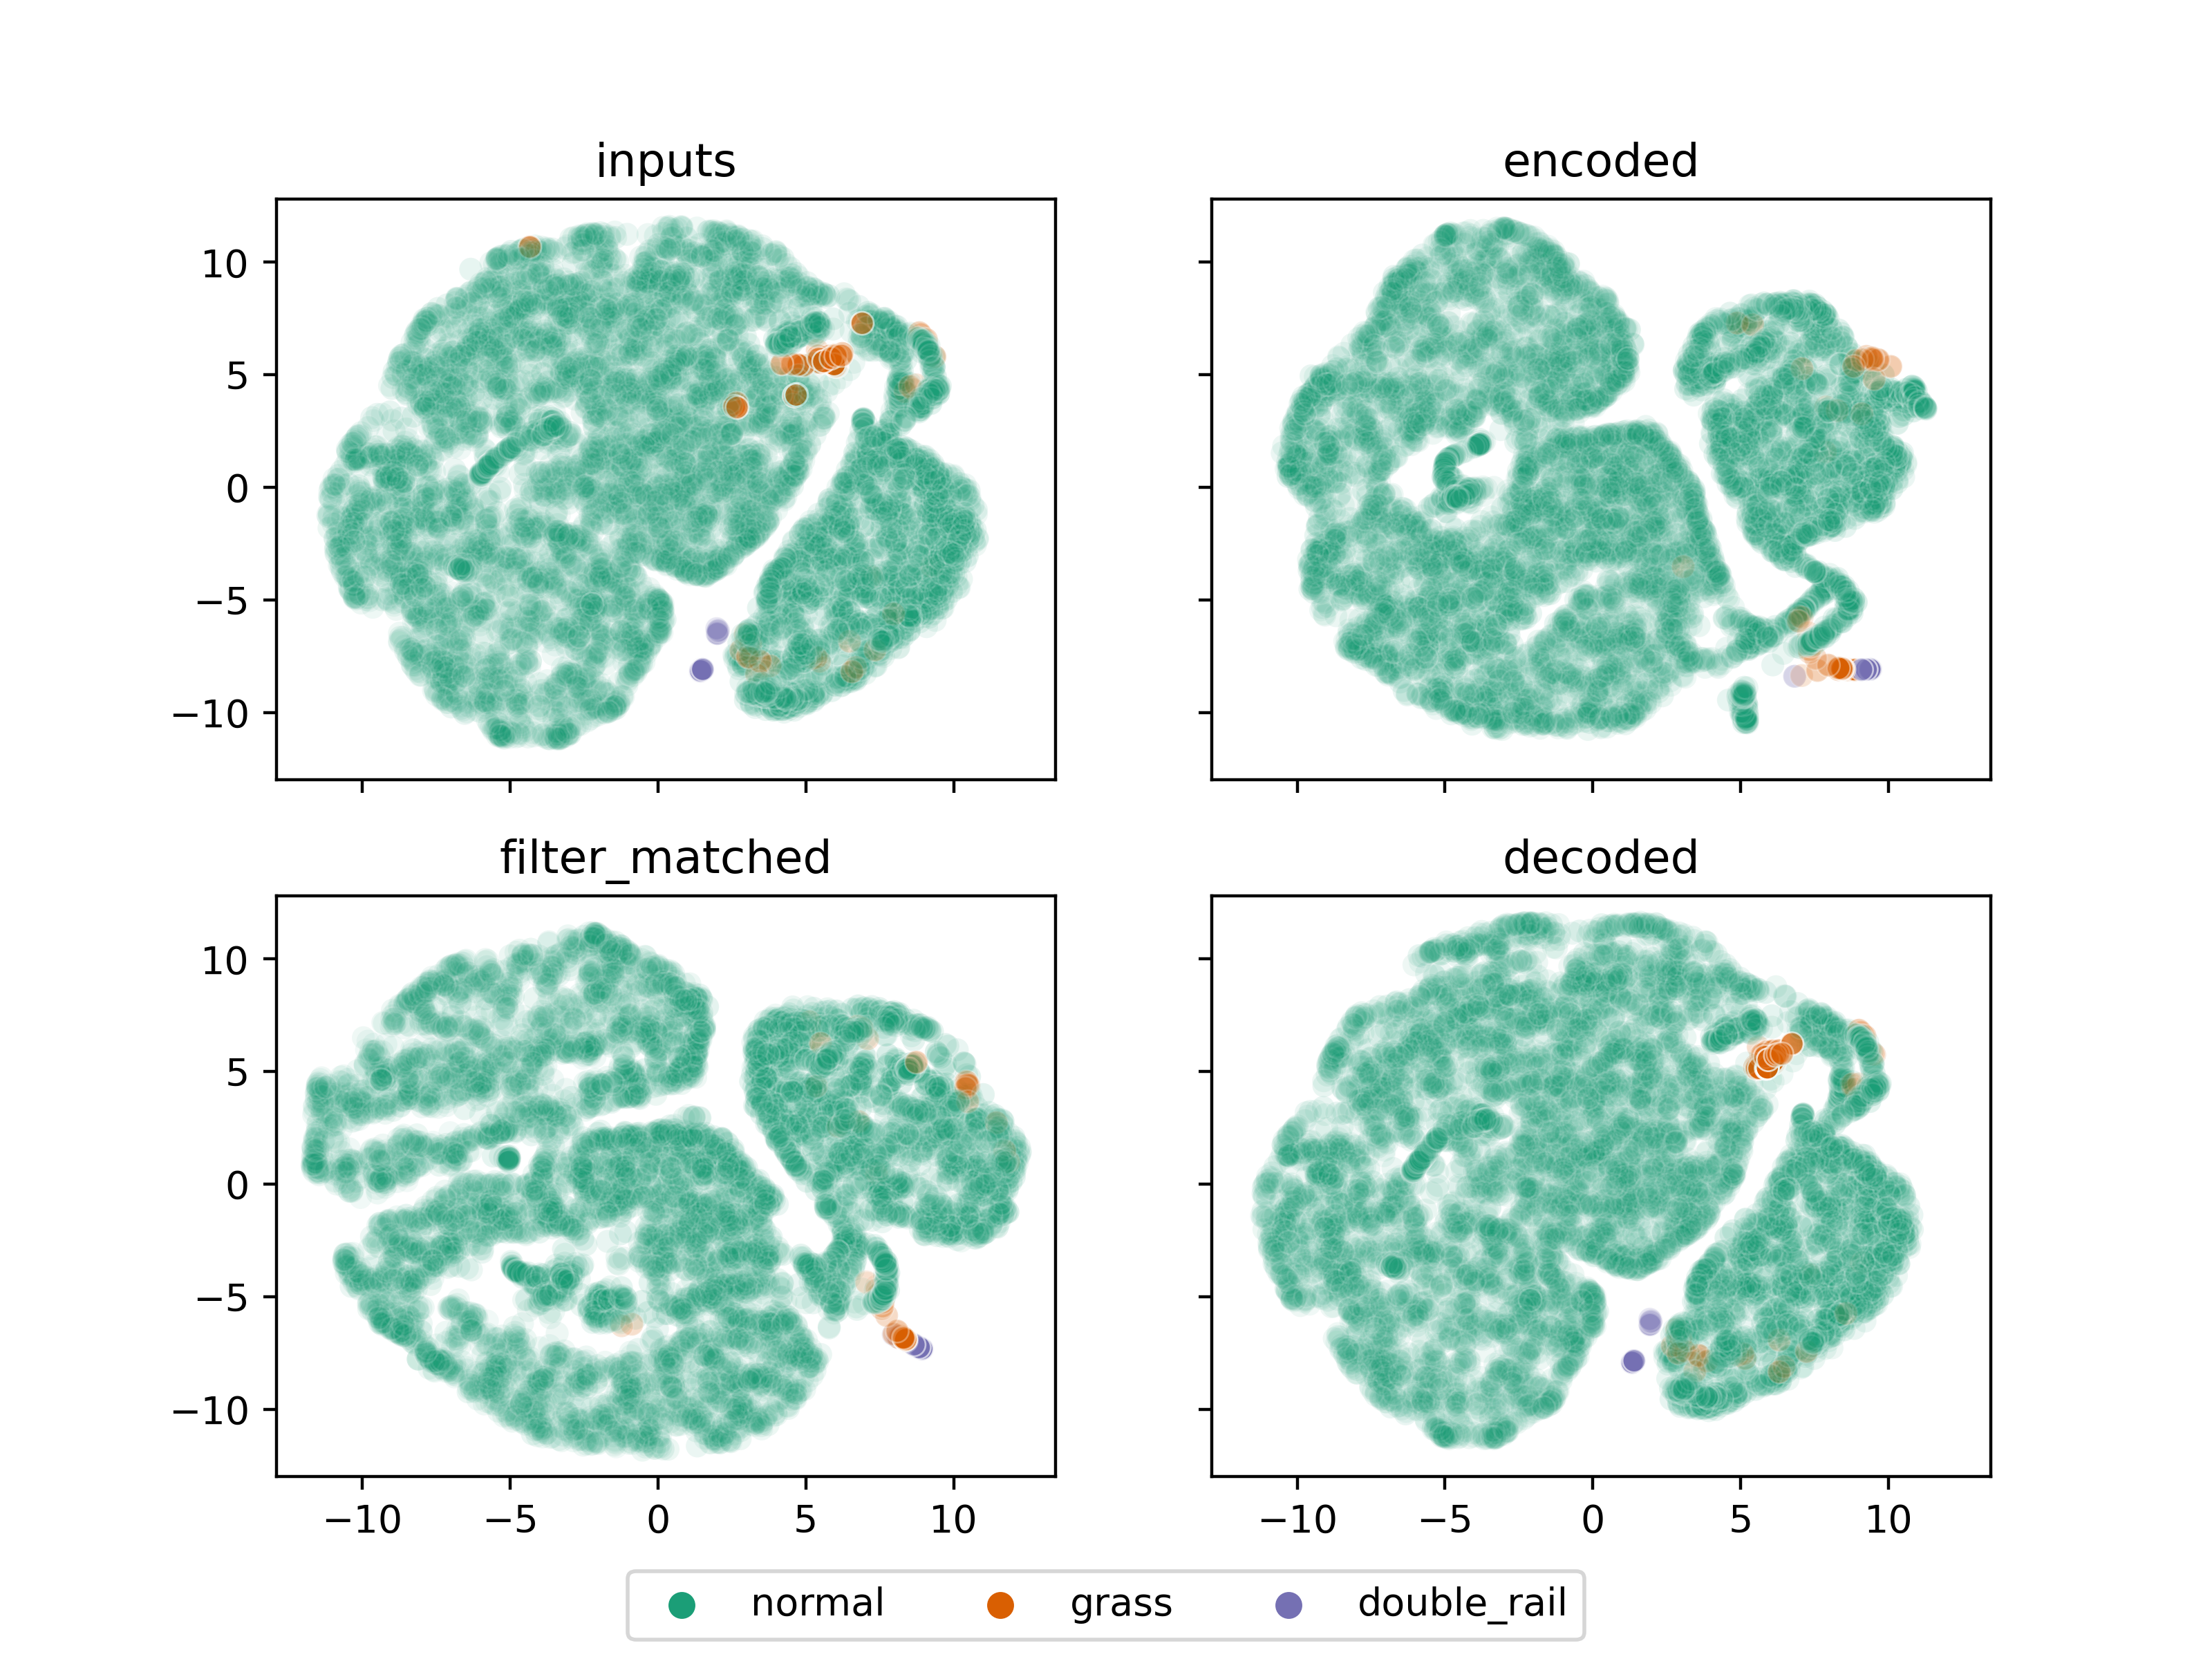
\includegraphics[width=\columnwidth,trim={0 0 0 1cm},clip]{./results/resnet50_vgg19/20230514_213740_feature_vectors_1.png}
                \caption*{ResNet50}
            \end{figure}
        \end{column}
        \begin{column}{0.45\textwidth}
            \begin{figure}
                \centering
                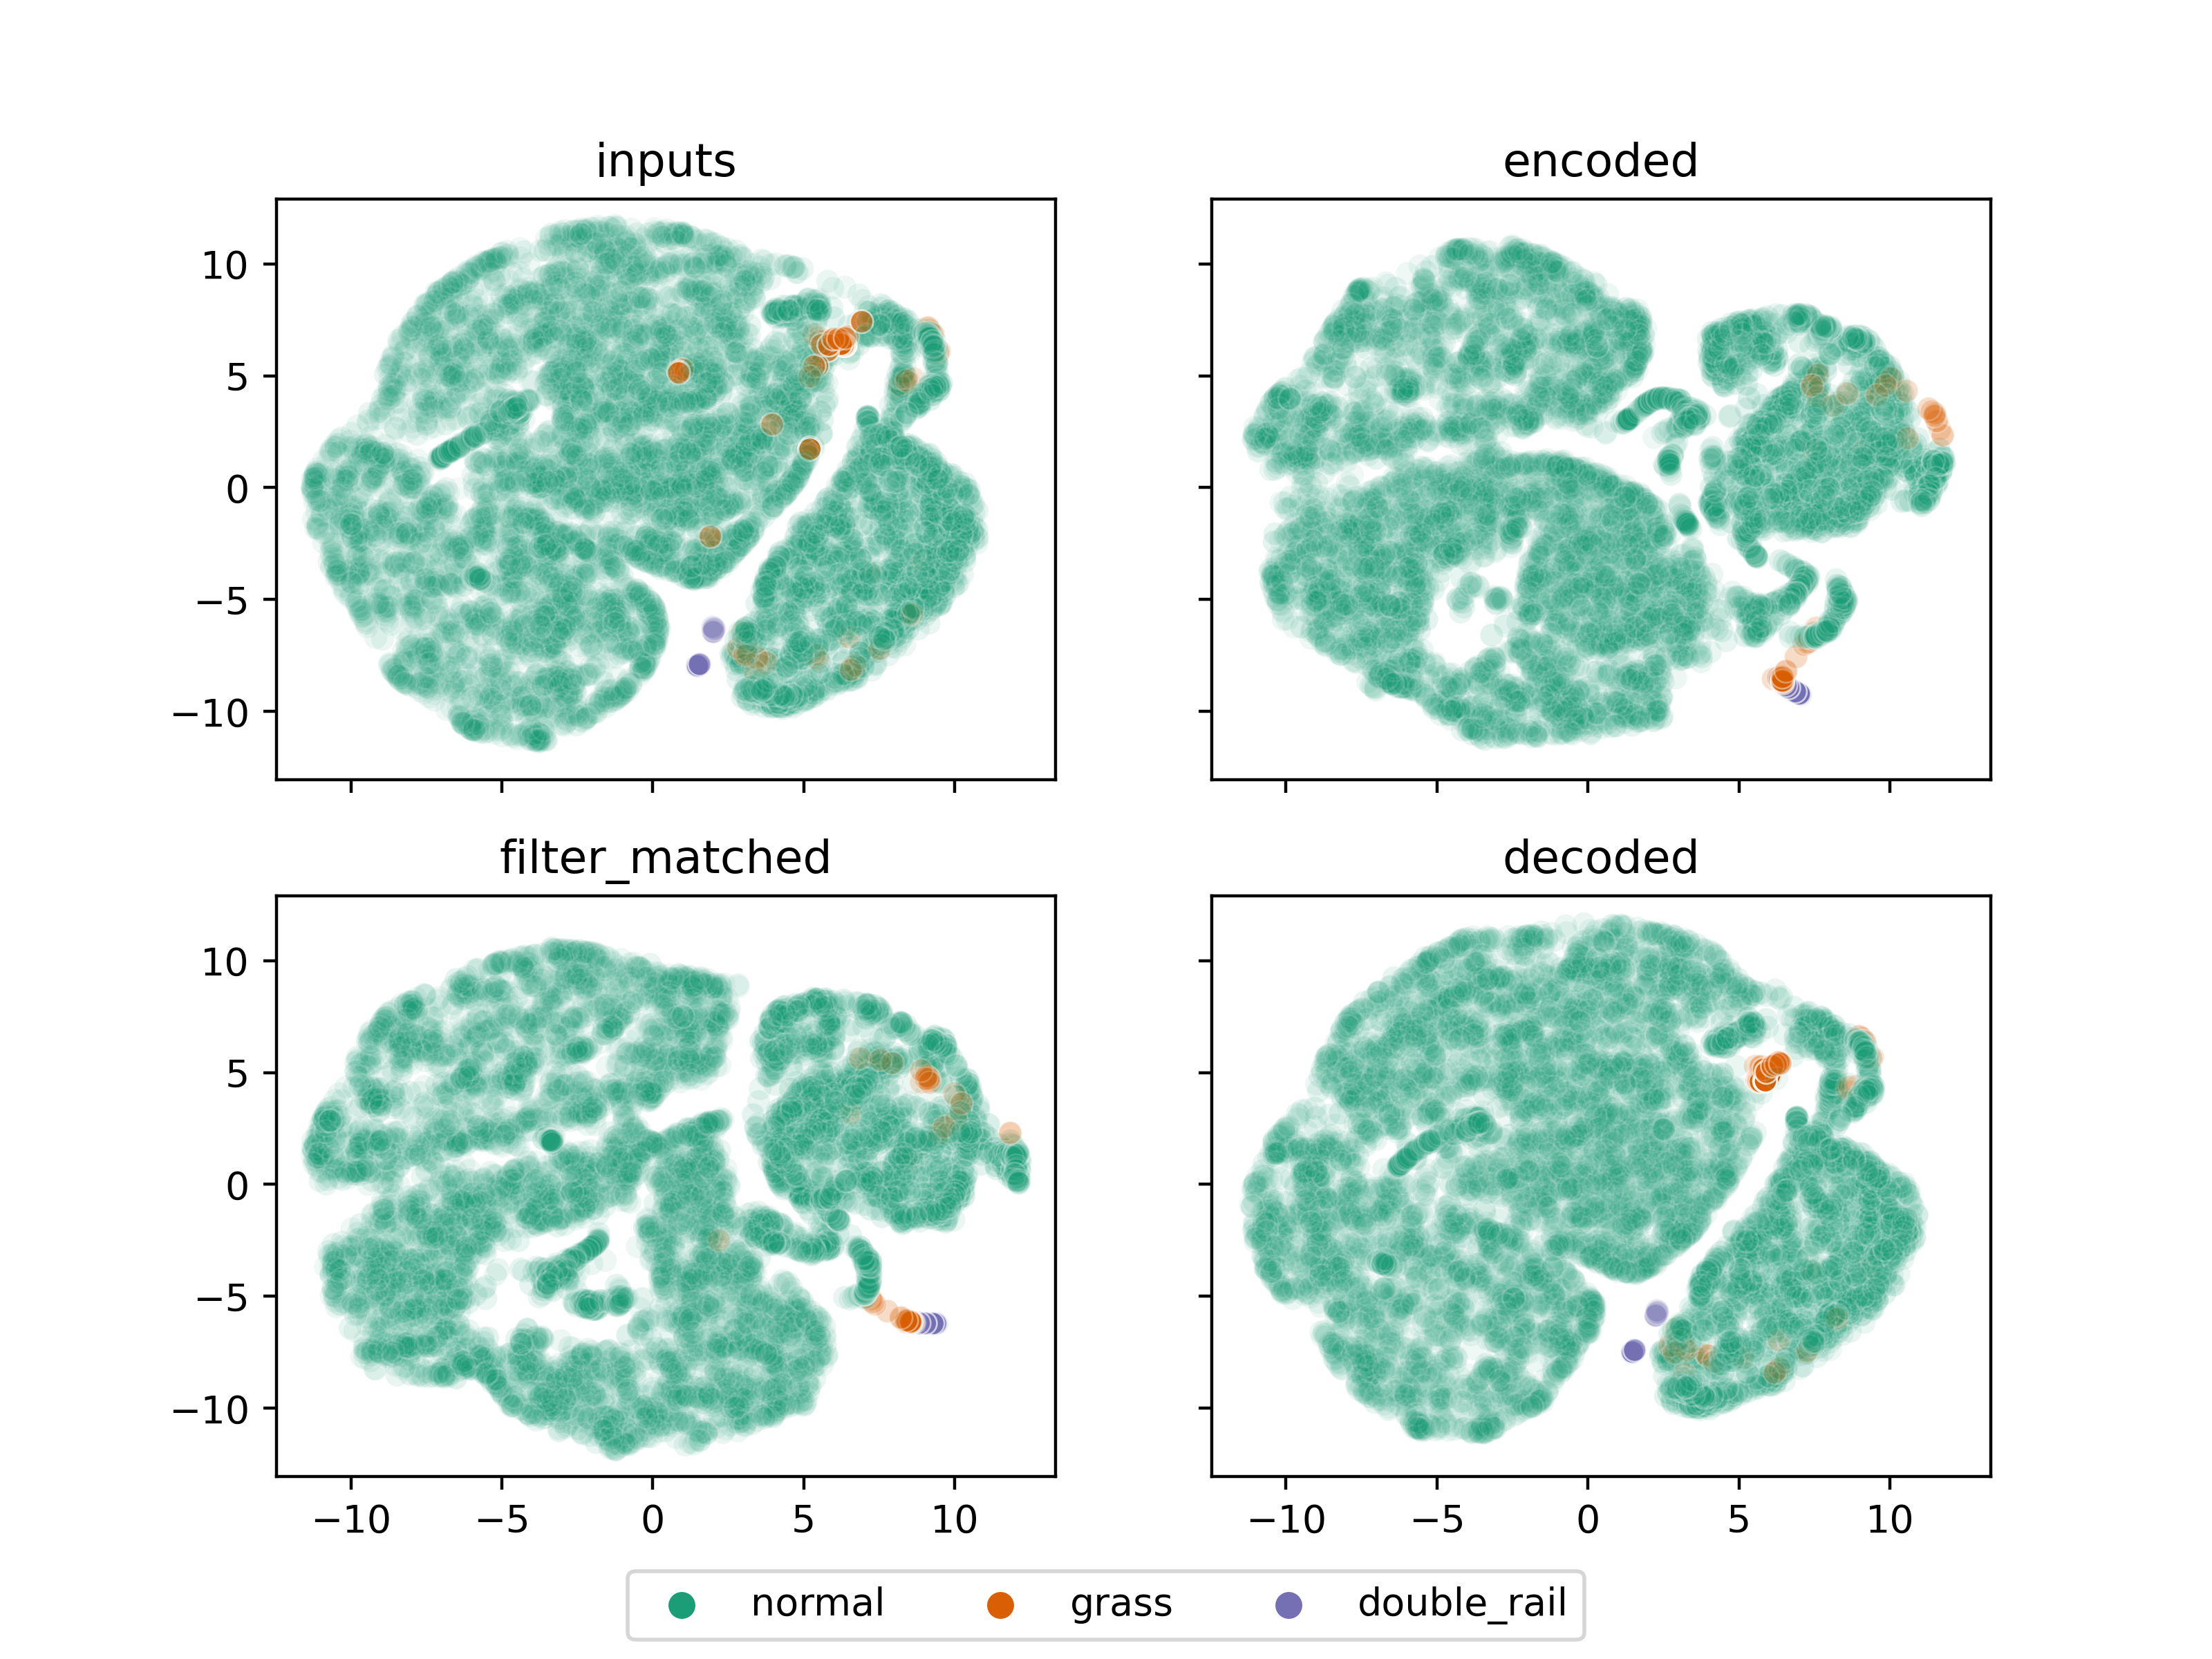
\includegraphics[width=\columnwidth,trim={0 0 0 1cm},clip]{./results/efficientnetv2l_vgg19/20230525_194238_feature_vectors_1.png}
                \caption*{EfficientNetV2L}
            \end{figure}
        \end{column}
    \end{columns}
\end{frame}

\begin{frame}{Loss based outliers}
    \begin{columns}
        \begin{column}{0.45\textwidth}
            \begin{figure}
                \centering
                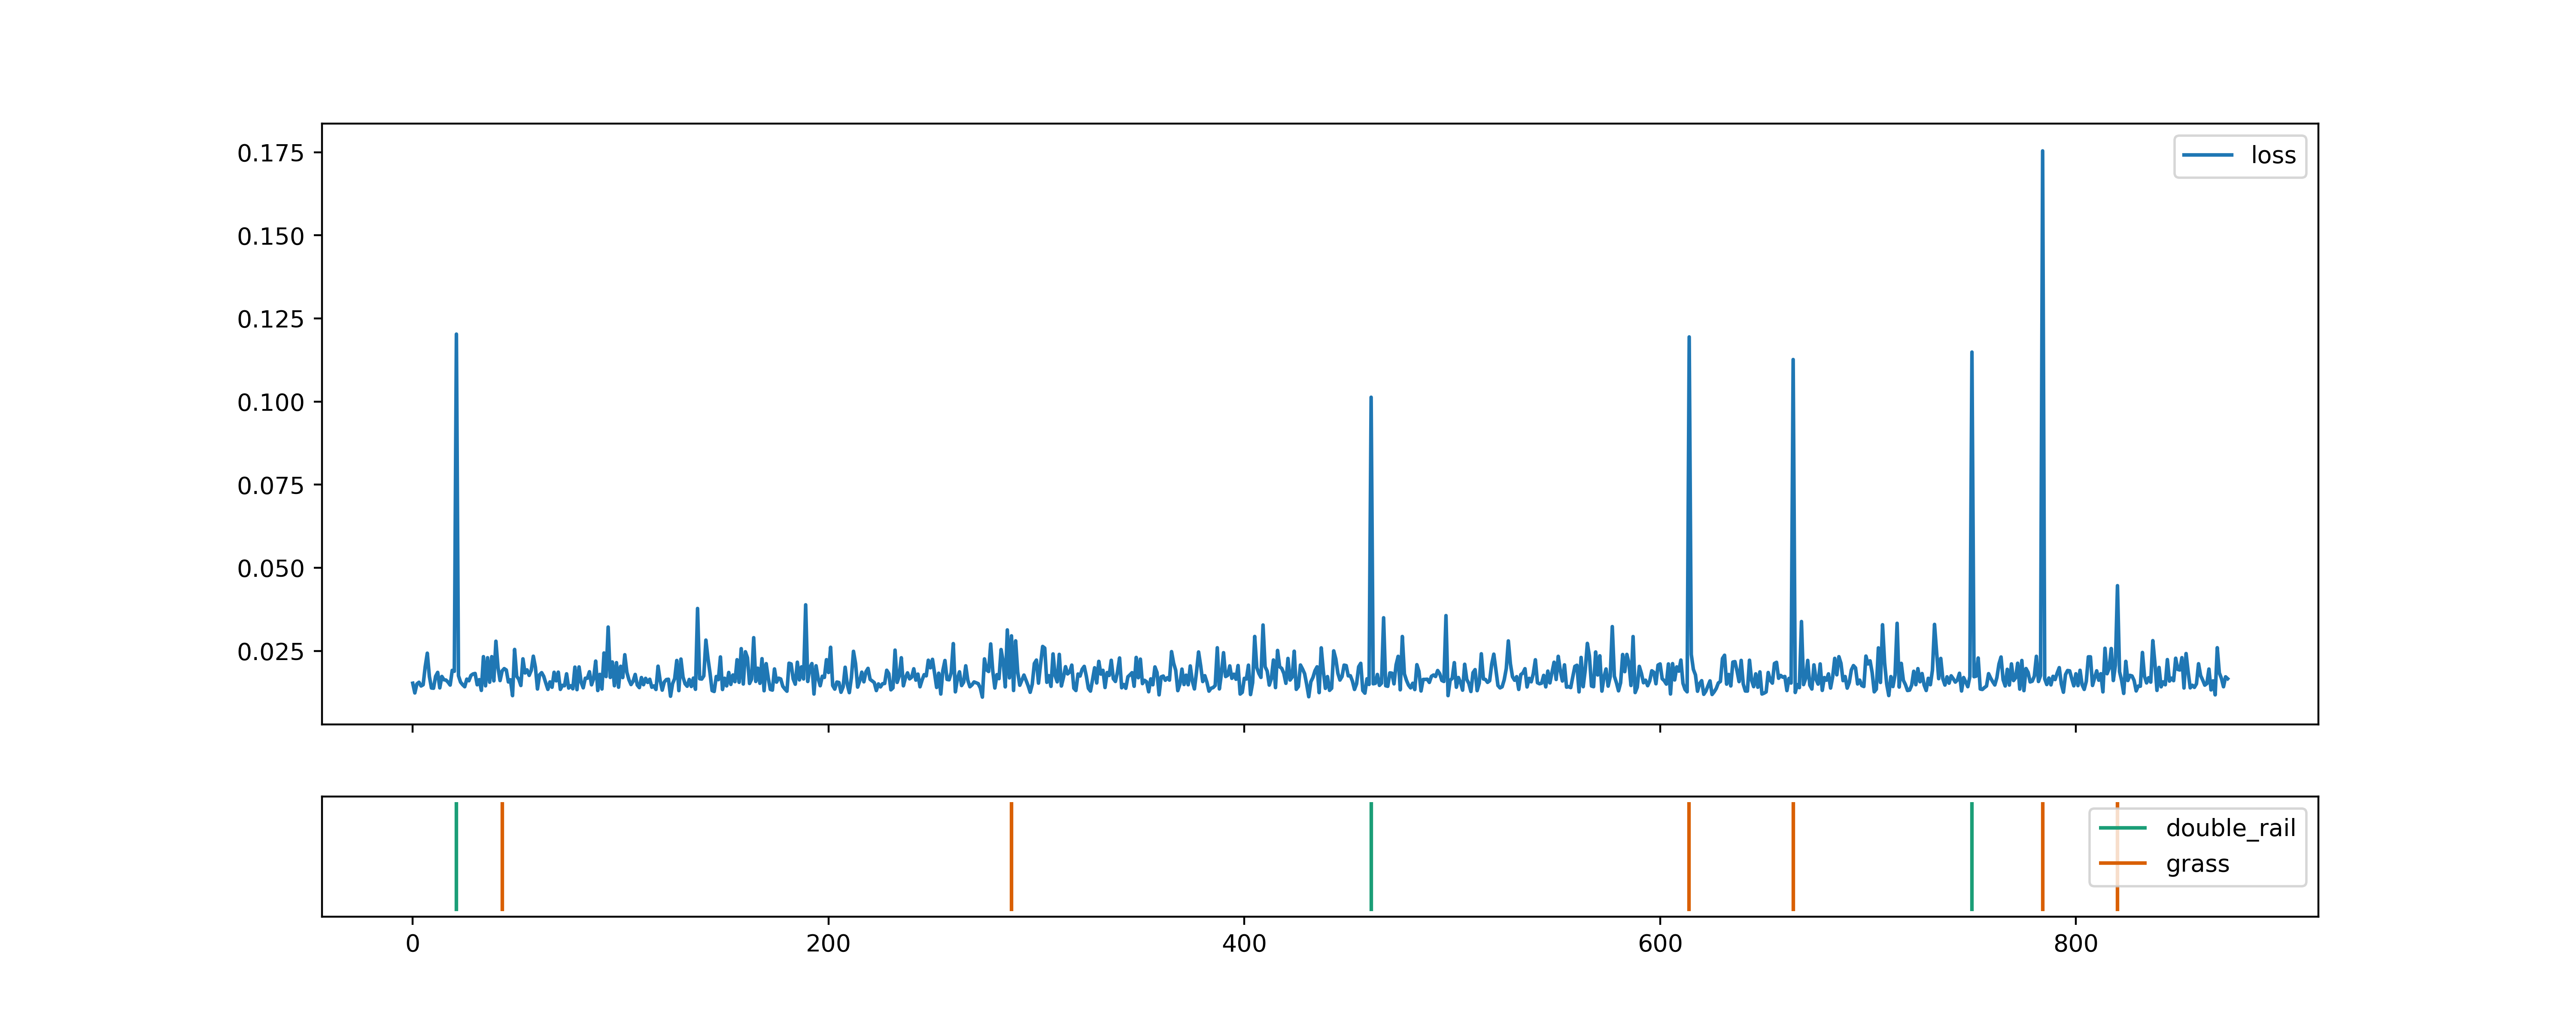
\includegraphics[width=\columnwidth,trim={0 0 0 1cm},clip]{./results/vgg19_vgg19/20230510_172958_feature_vectors_loss.png}
                \caption*{VGG19}
                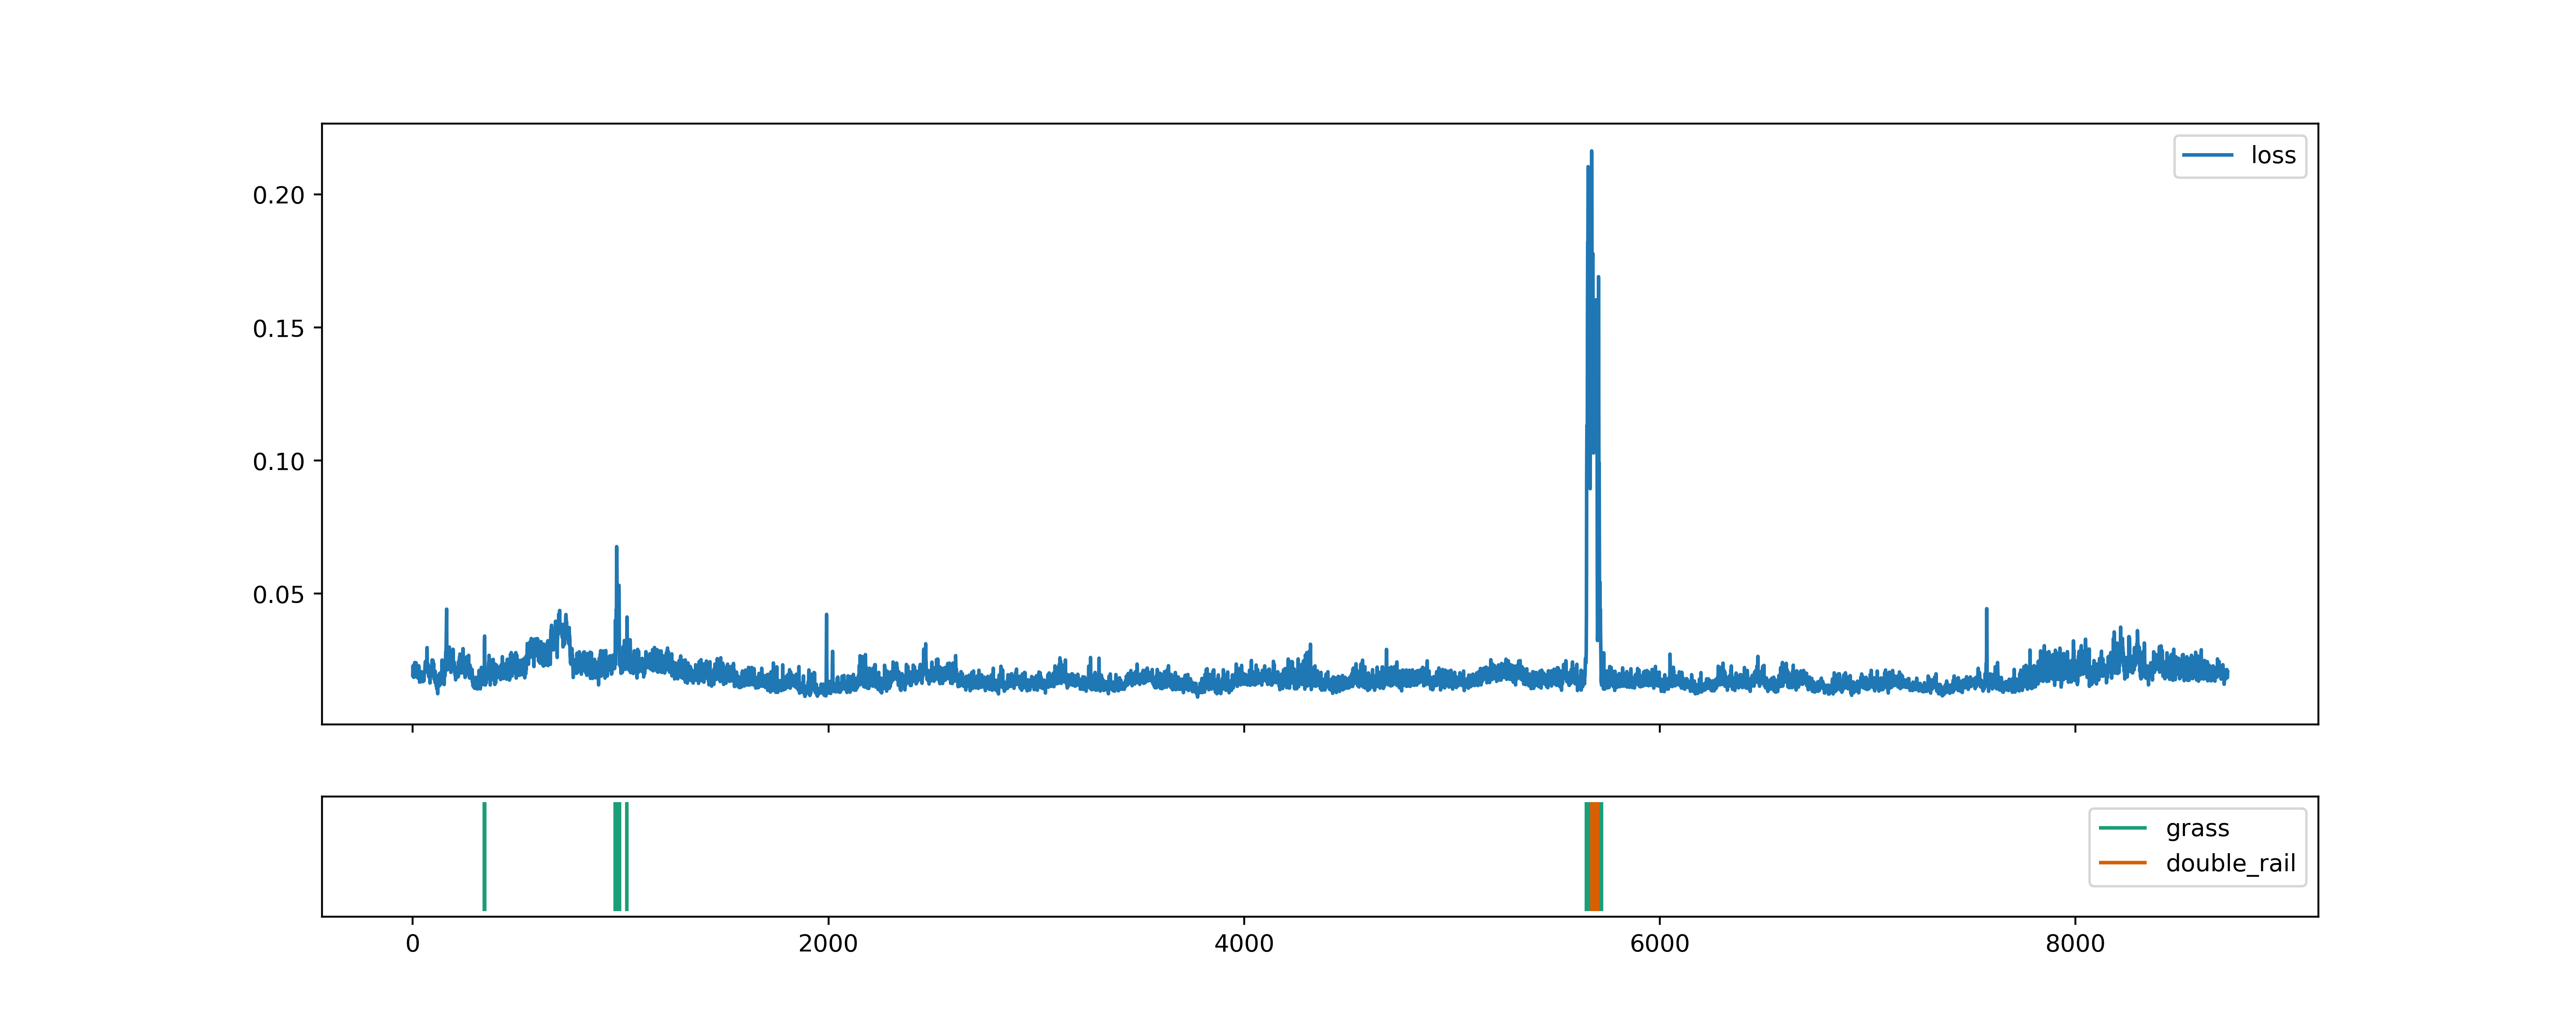
\includegraphics[width=\columnwidth,trim={0 0 0 1cm},clip]{./results/resnet50_vgg19/20230514_213740_feature_vectors_loss.png}
                \caption*{ResNet50}
            \end{figure}
        \end{column}
        \begin{column}{0.45\textwidth}
            \begin{figure}
                \centering
                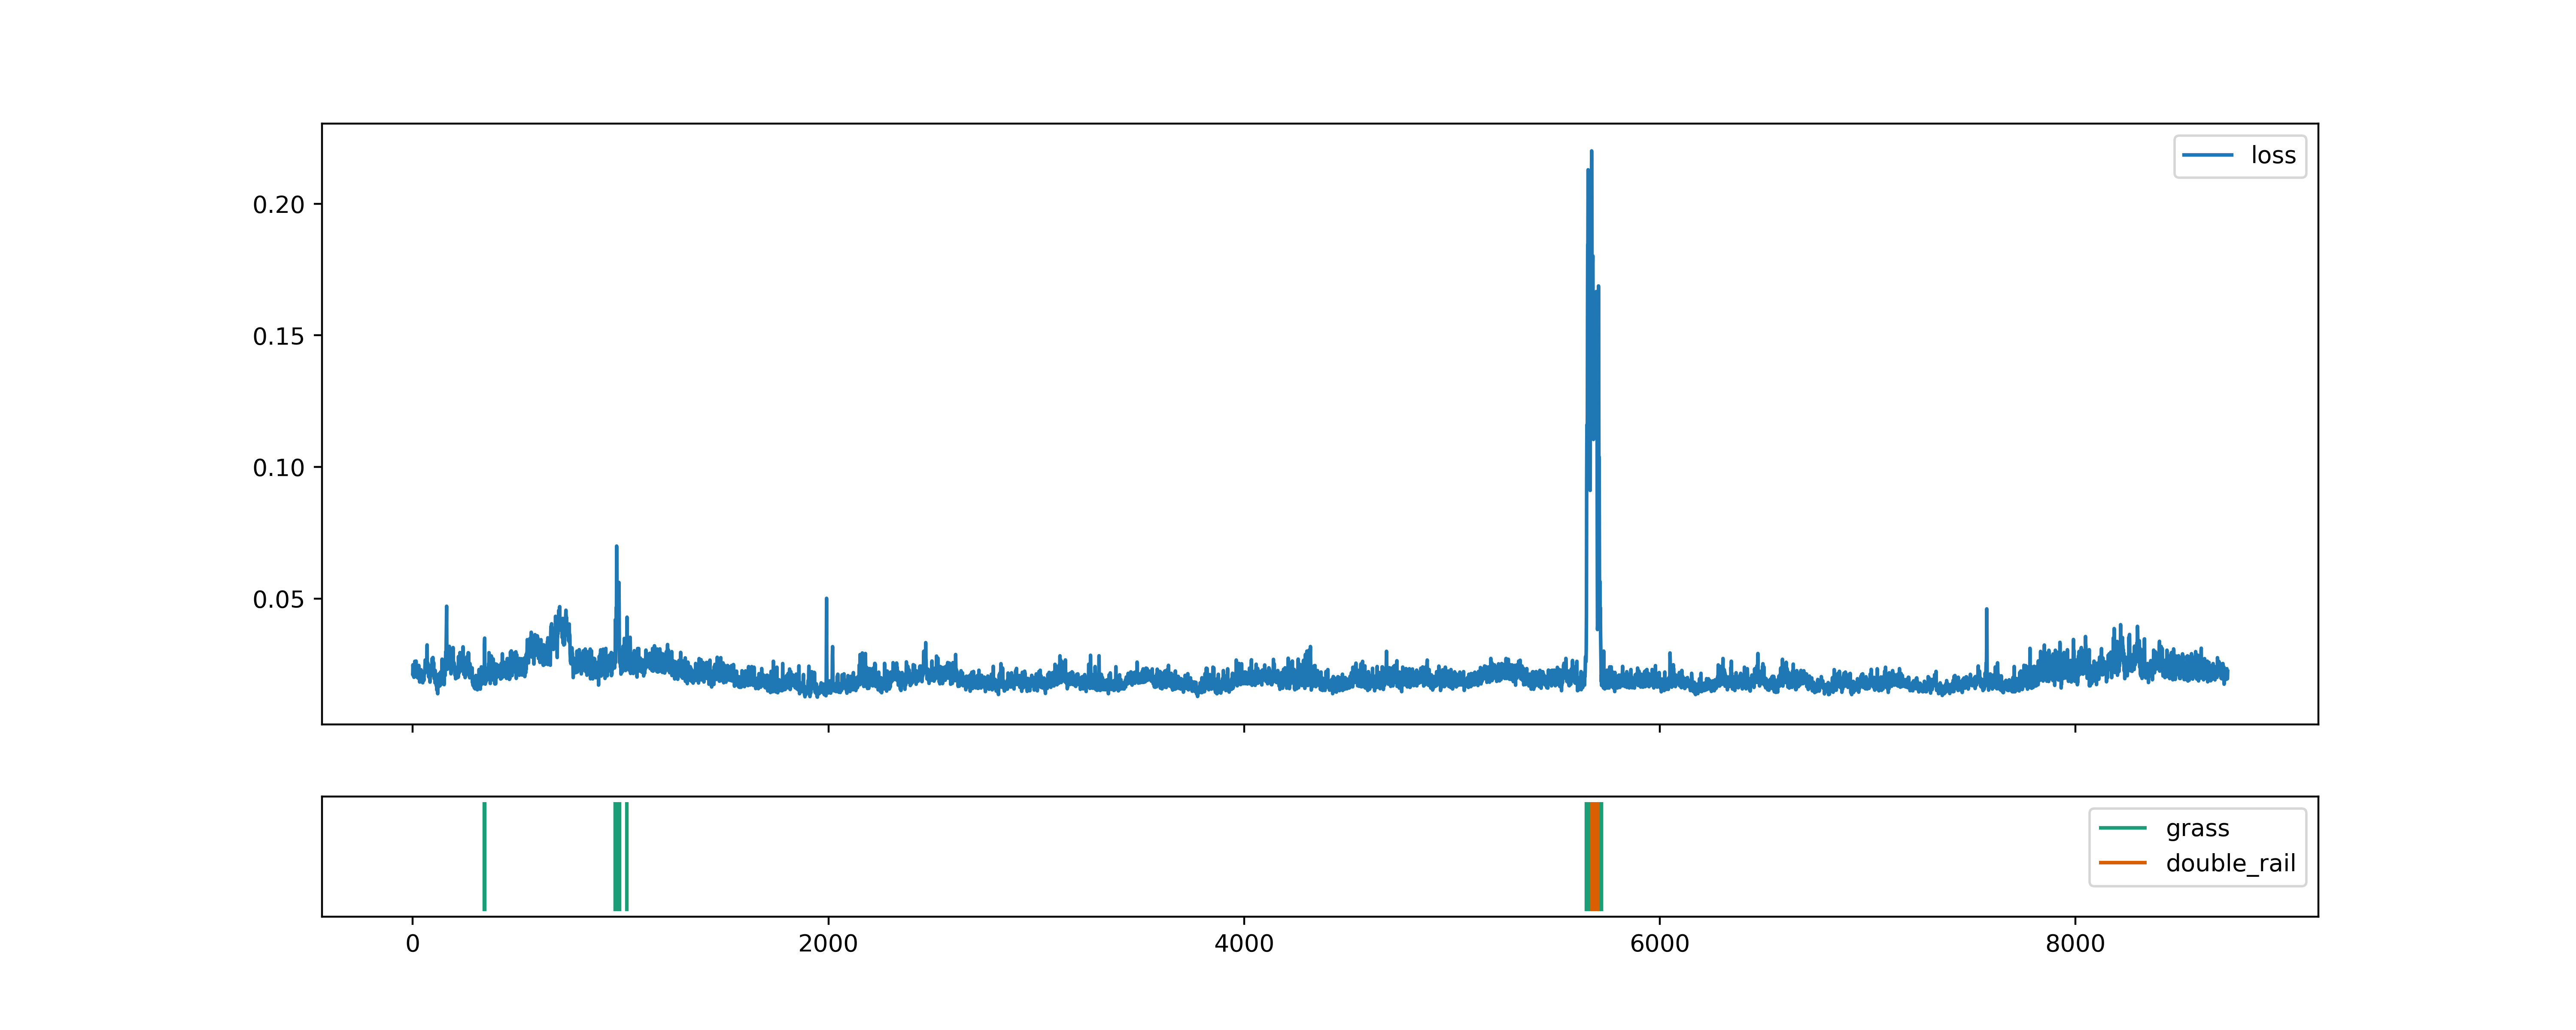
\includegraphics[width=\columnwidth,trim={0 0 0 1cm},clip]{./results/vgg19_bn_vgg19/20230525_045131_feature_vectors_loss.png}
                \caption*{VGG19 BN}
                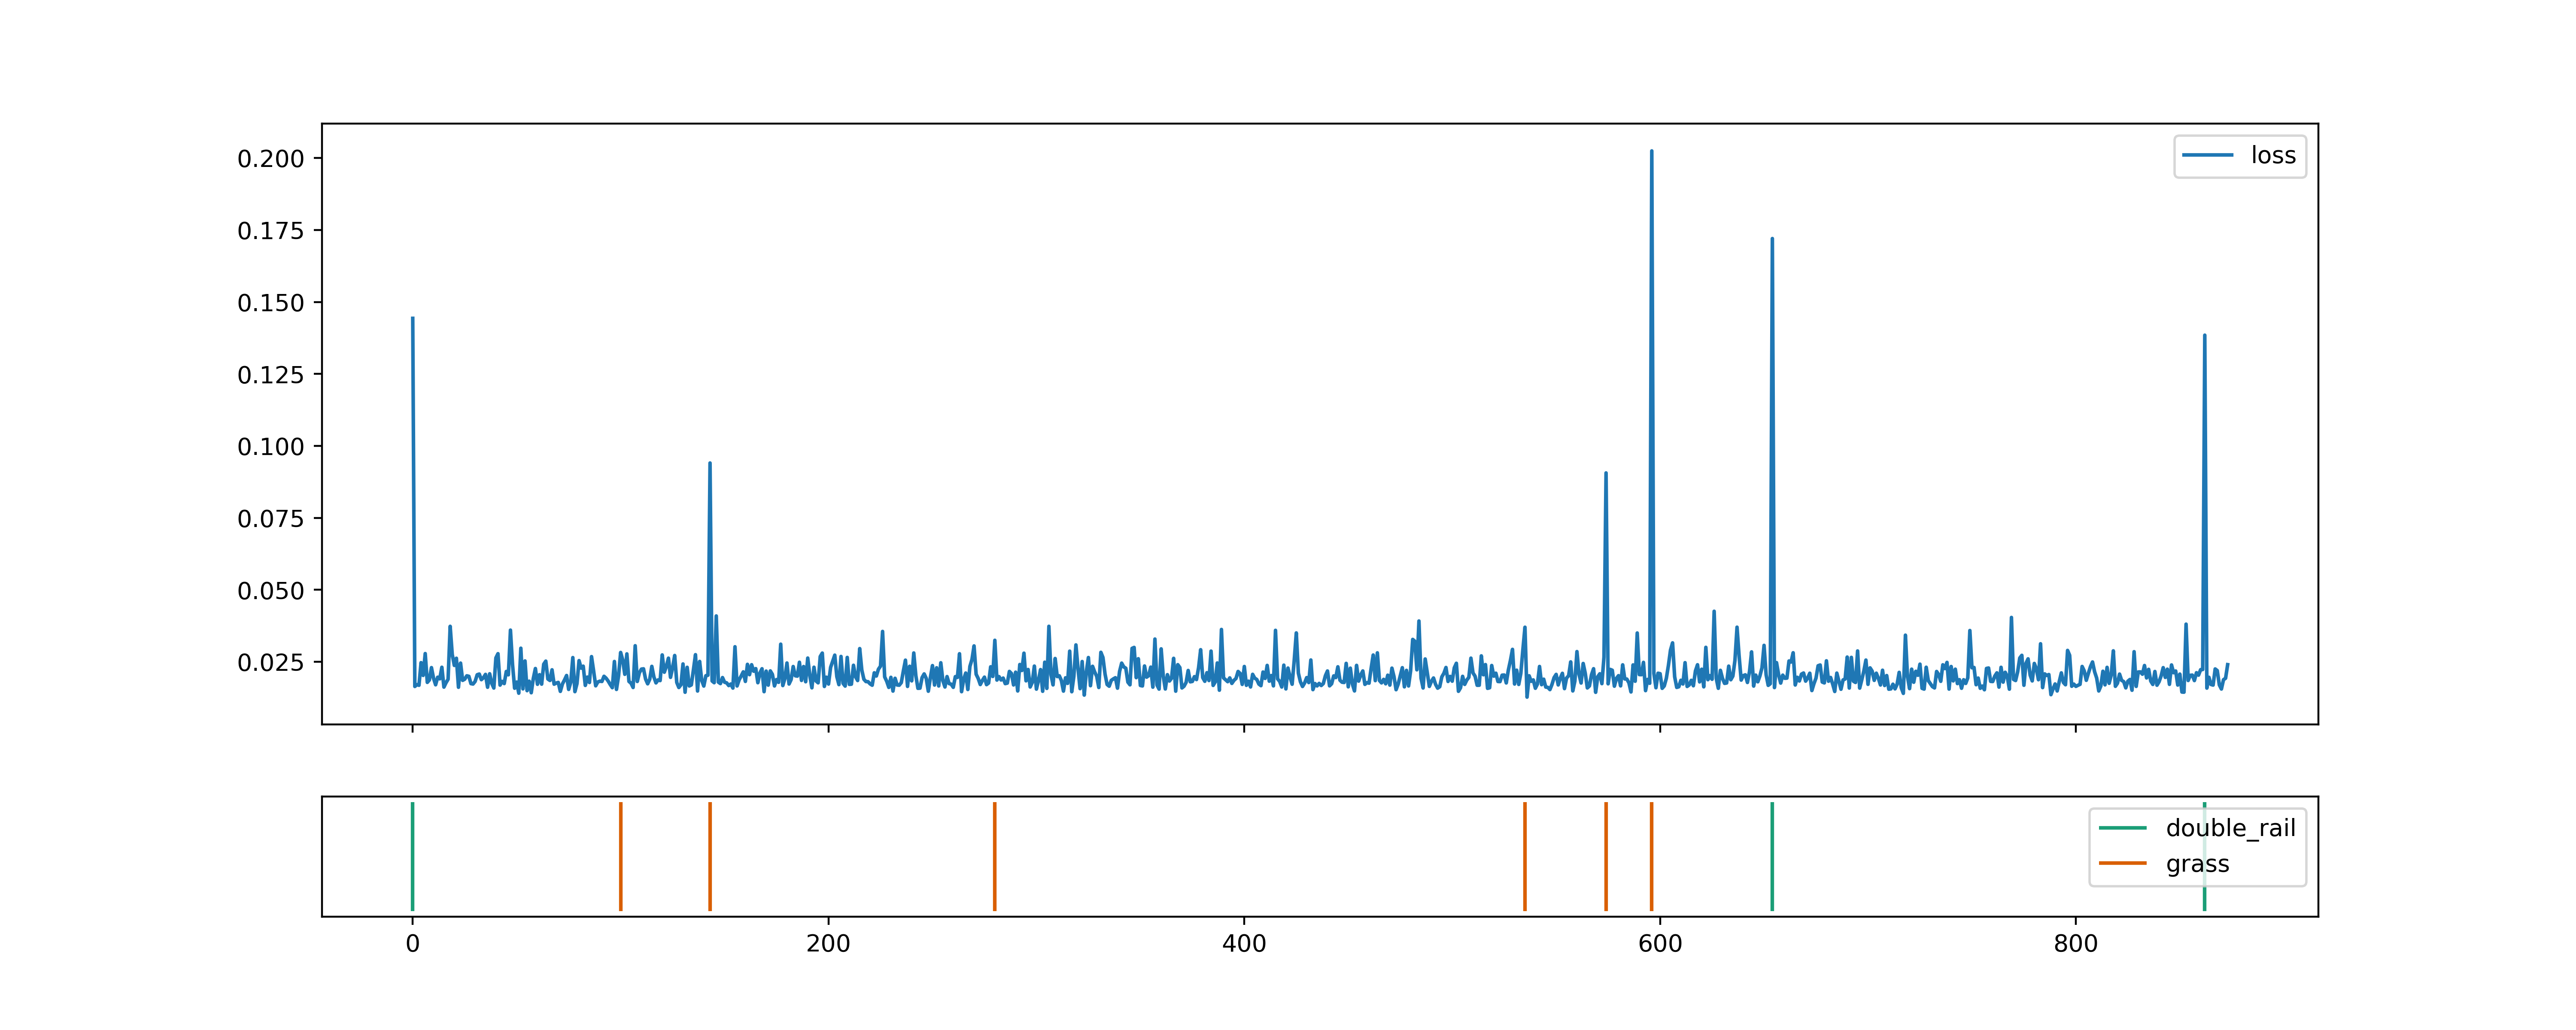
\includegraphics[width=\columnwidth,trim={0 0 0 1cm},clip]{./results/efficientnetv2l_vgg19/20230525_194238_feature_vectors_loss.png}
                \caption*{EfficientNetV2L}
            \end{figure}
        \end{column}
    \end{columns}
\end{frame}

\section{Discussion}
\begin{frame}{Learning curves}
    \begin{figure}
        \centering
        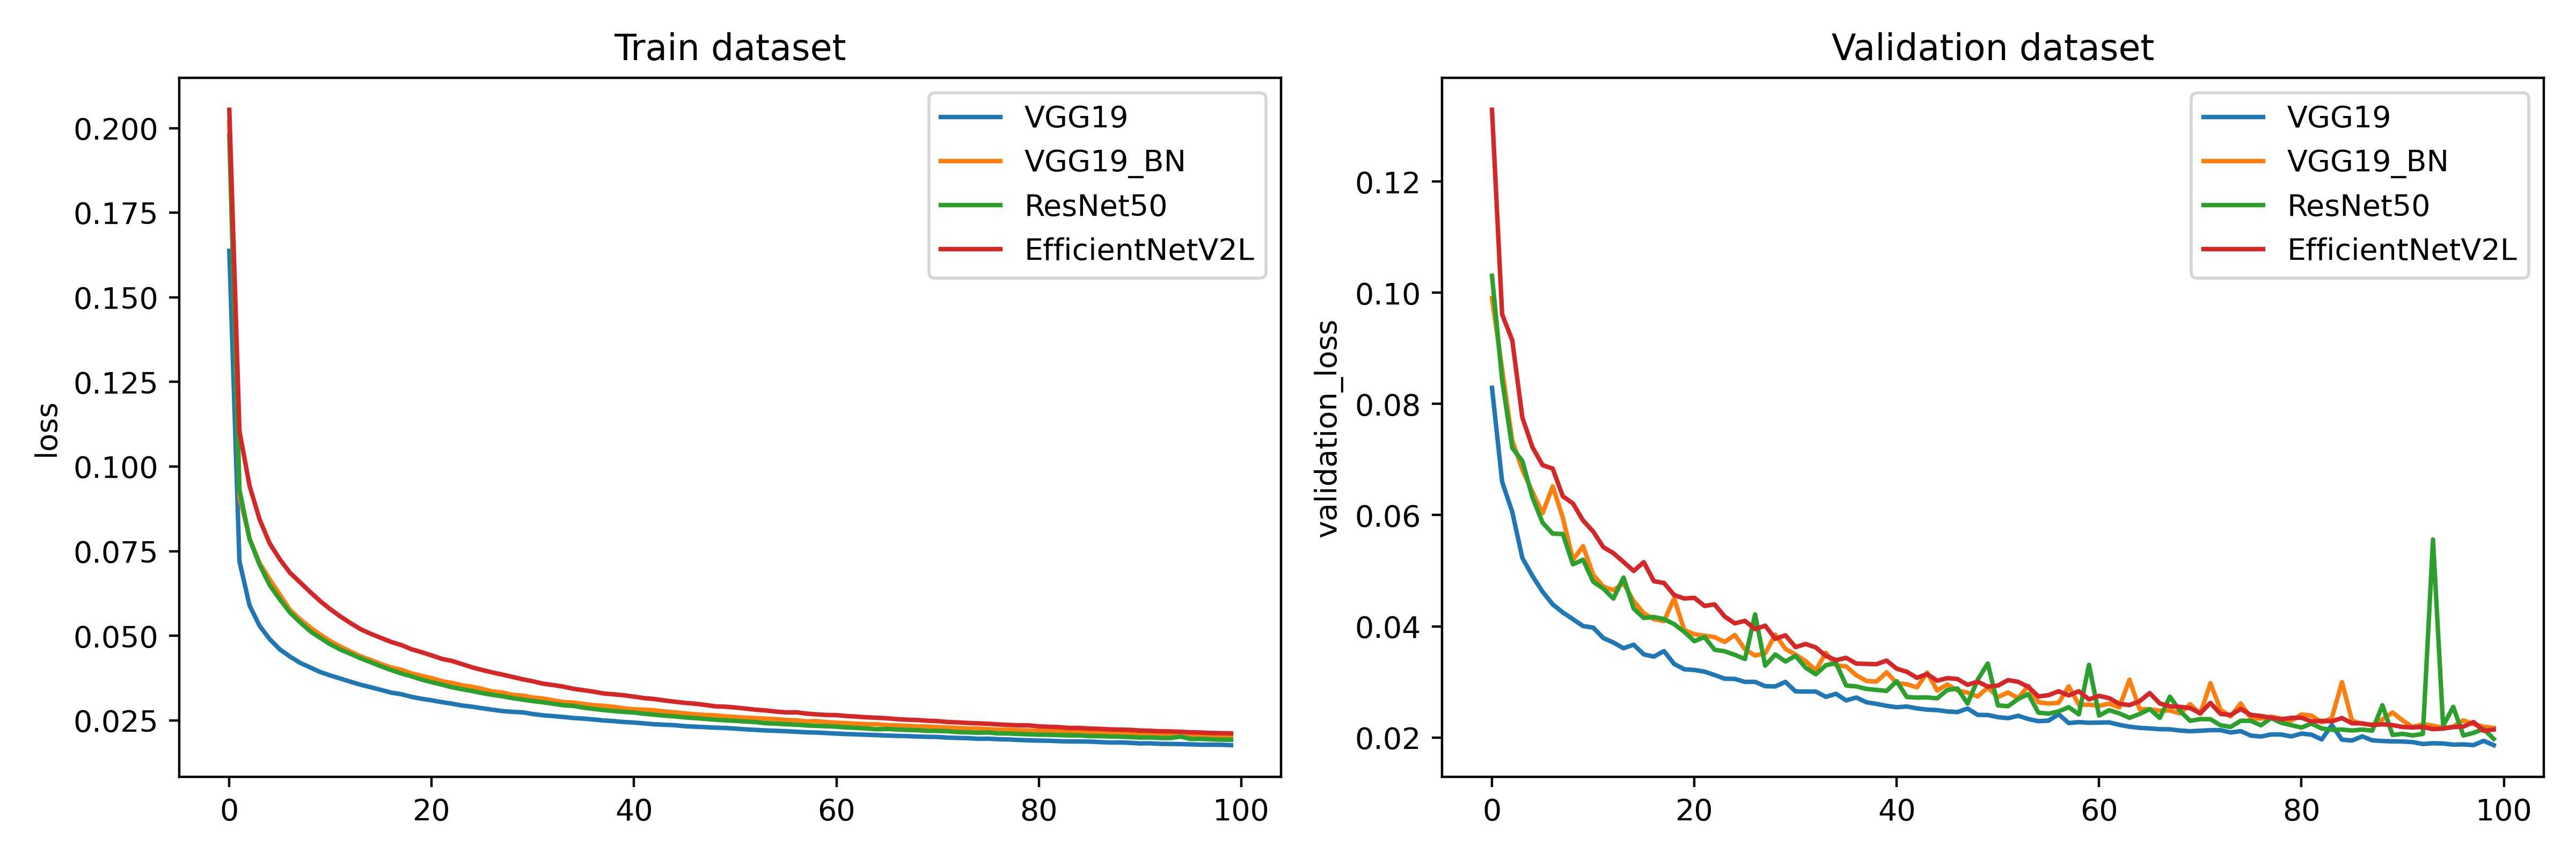
\includegraphics[width=\textwidth]{./results/comparison/learning_curves.png}
        \caption*{Learning curve comparison of different encoders}
    \end{figure}
\end{frame}

\begin{frame}{Loss-based threshold}
    \begin{columns}
        \begin{column}{0.45\textwidth}
            \begin{figure}
                \centering
                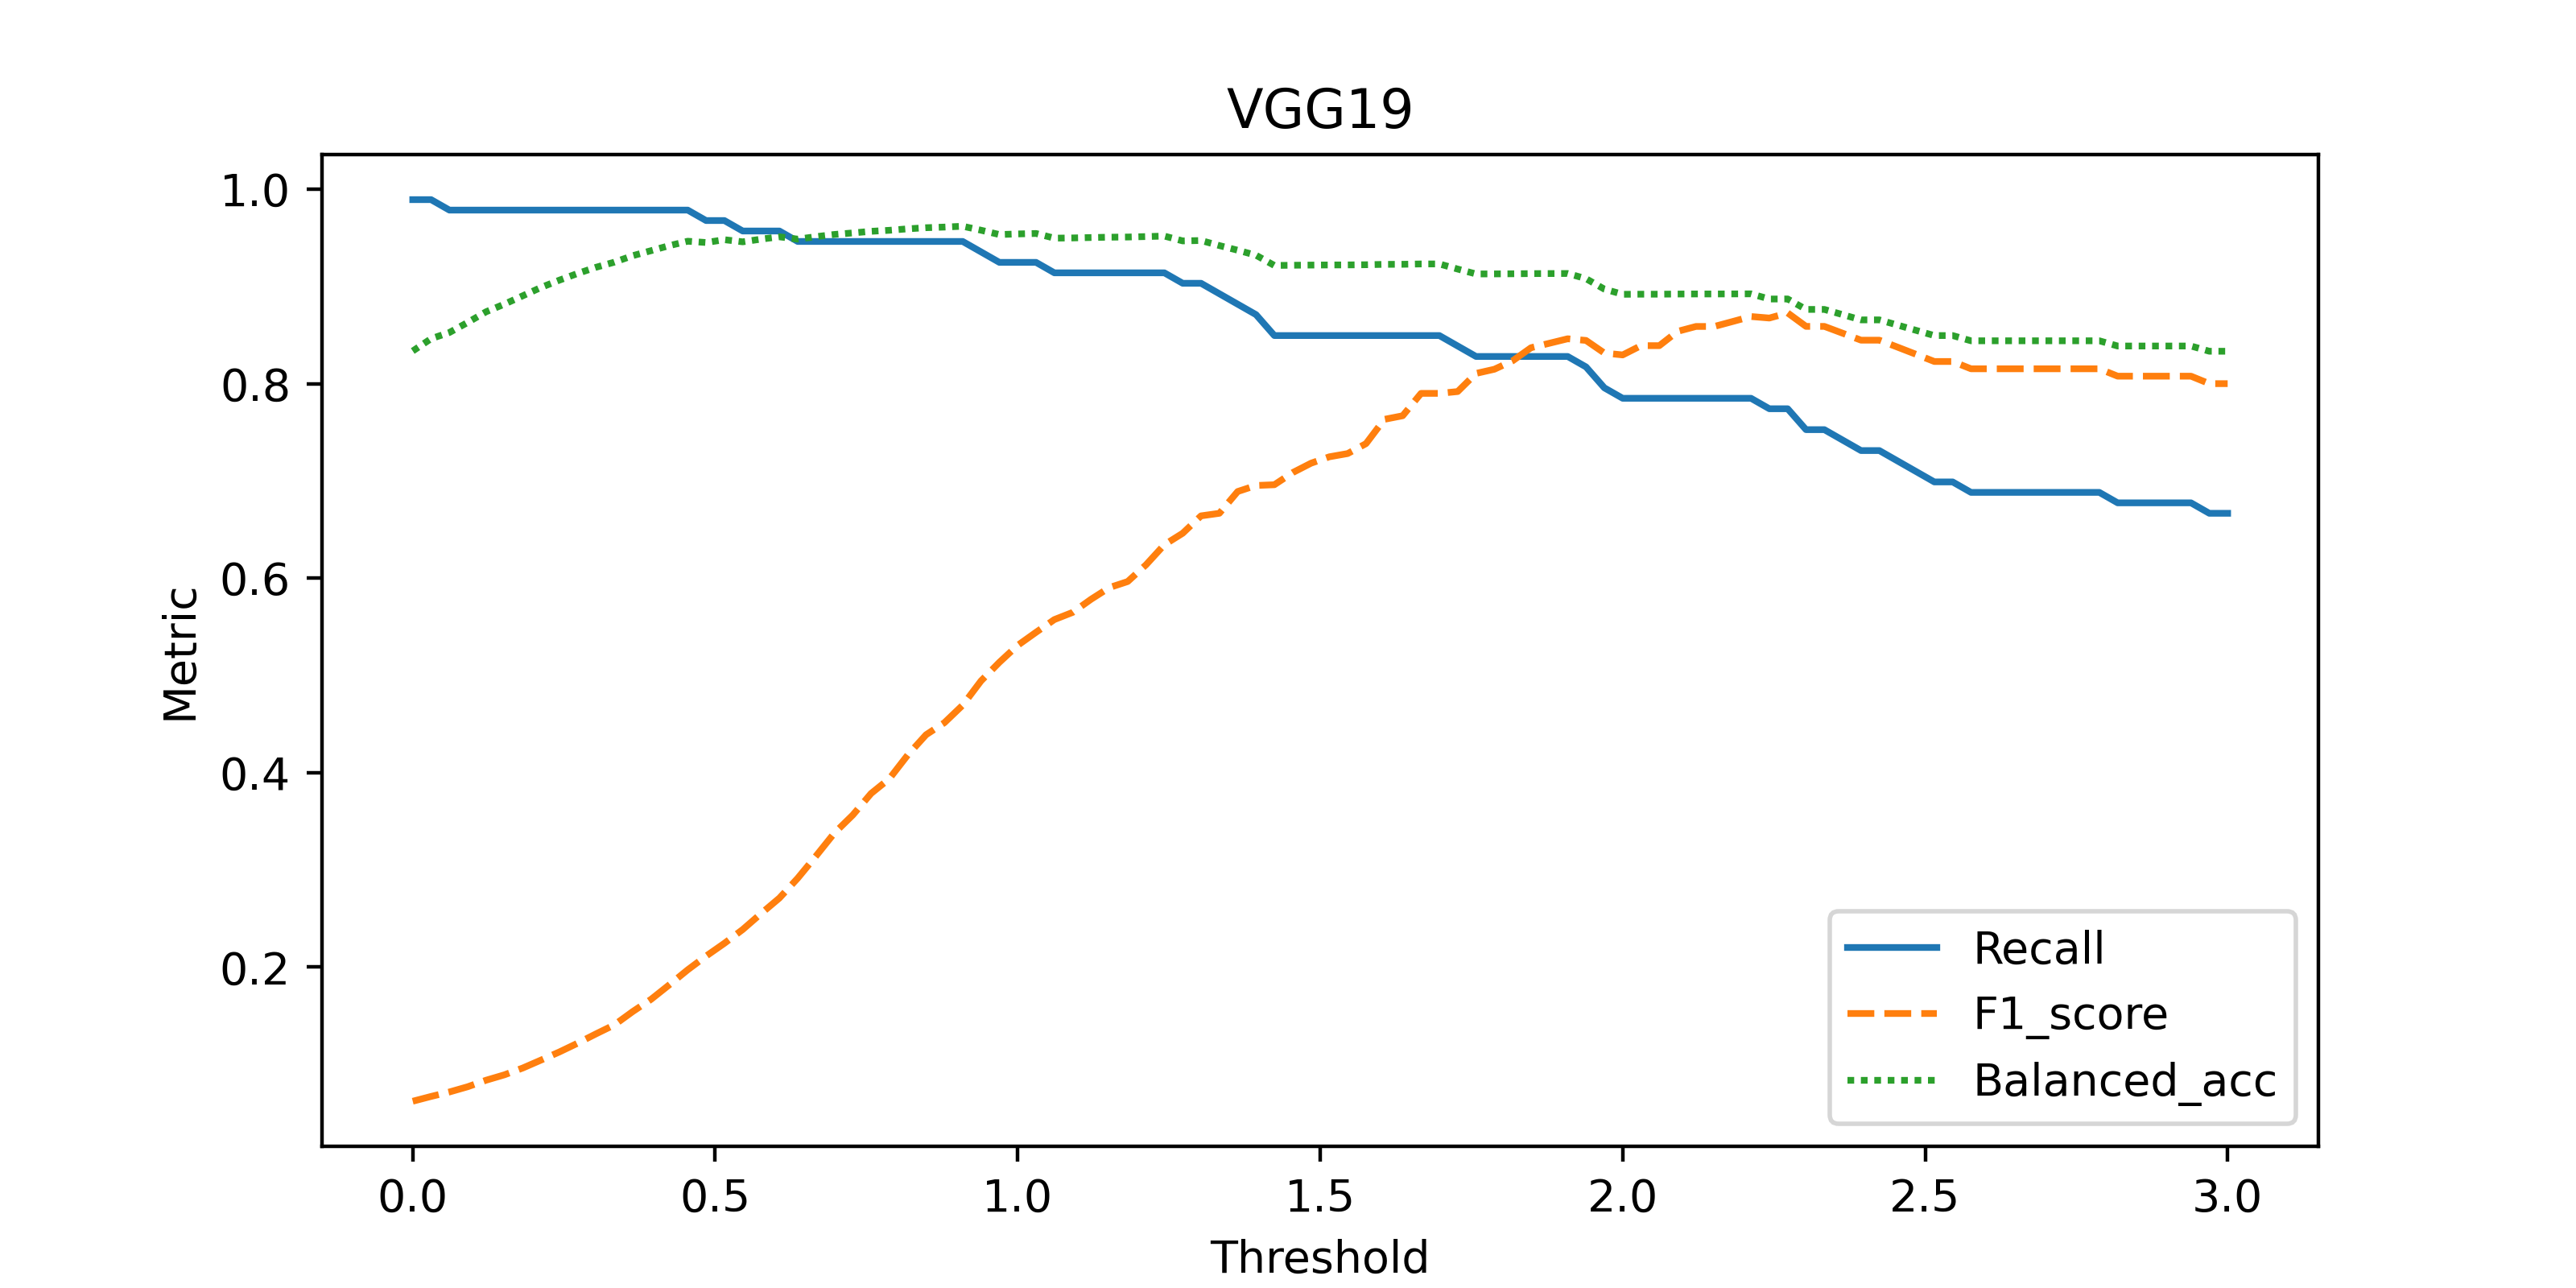
\includegraphics[width=\columnwidth]{./results/comparison/VGG19_threshold.png}
                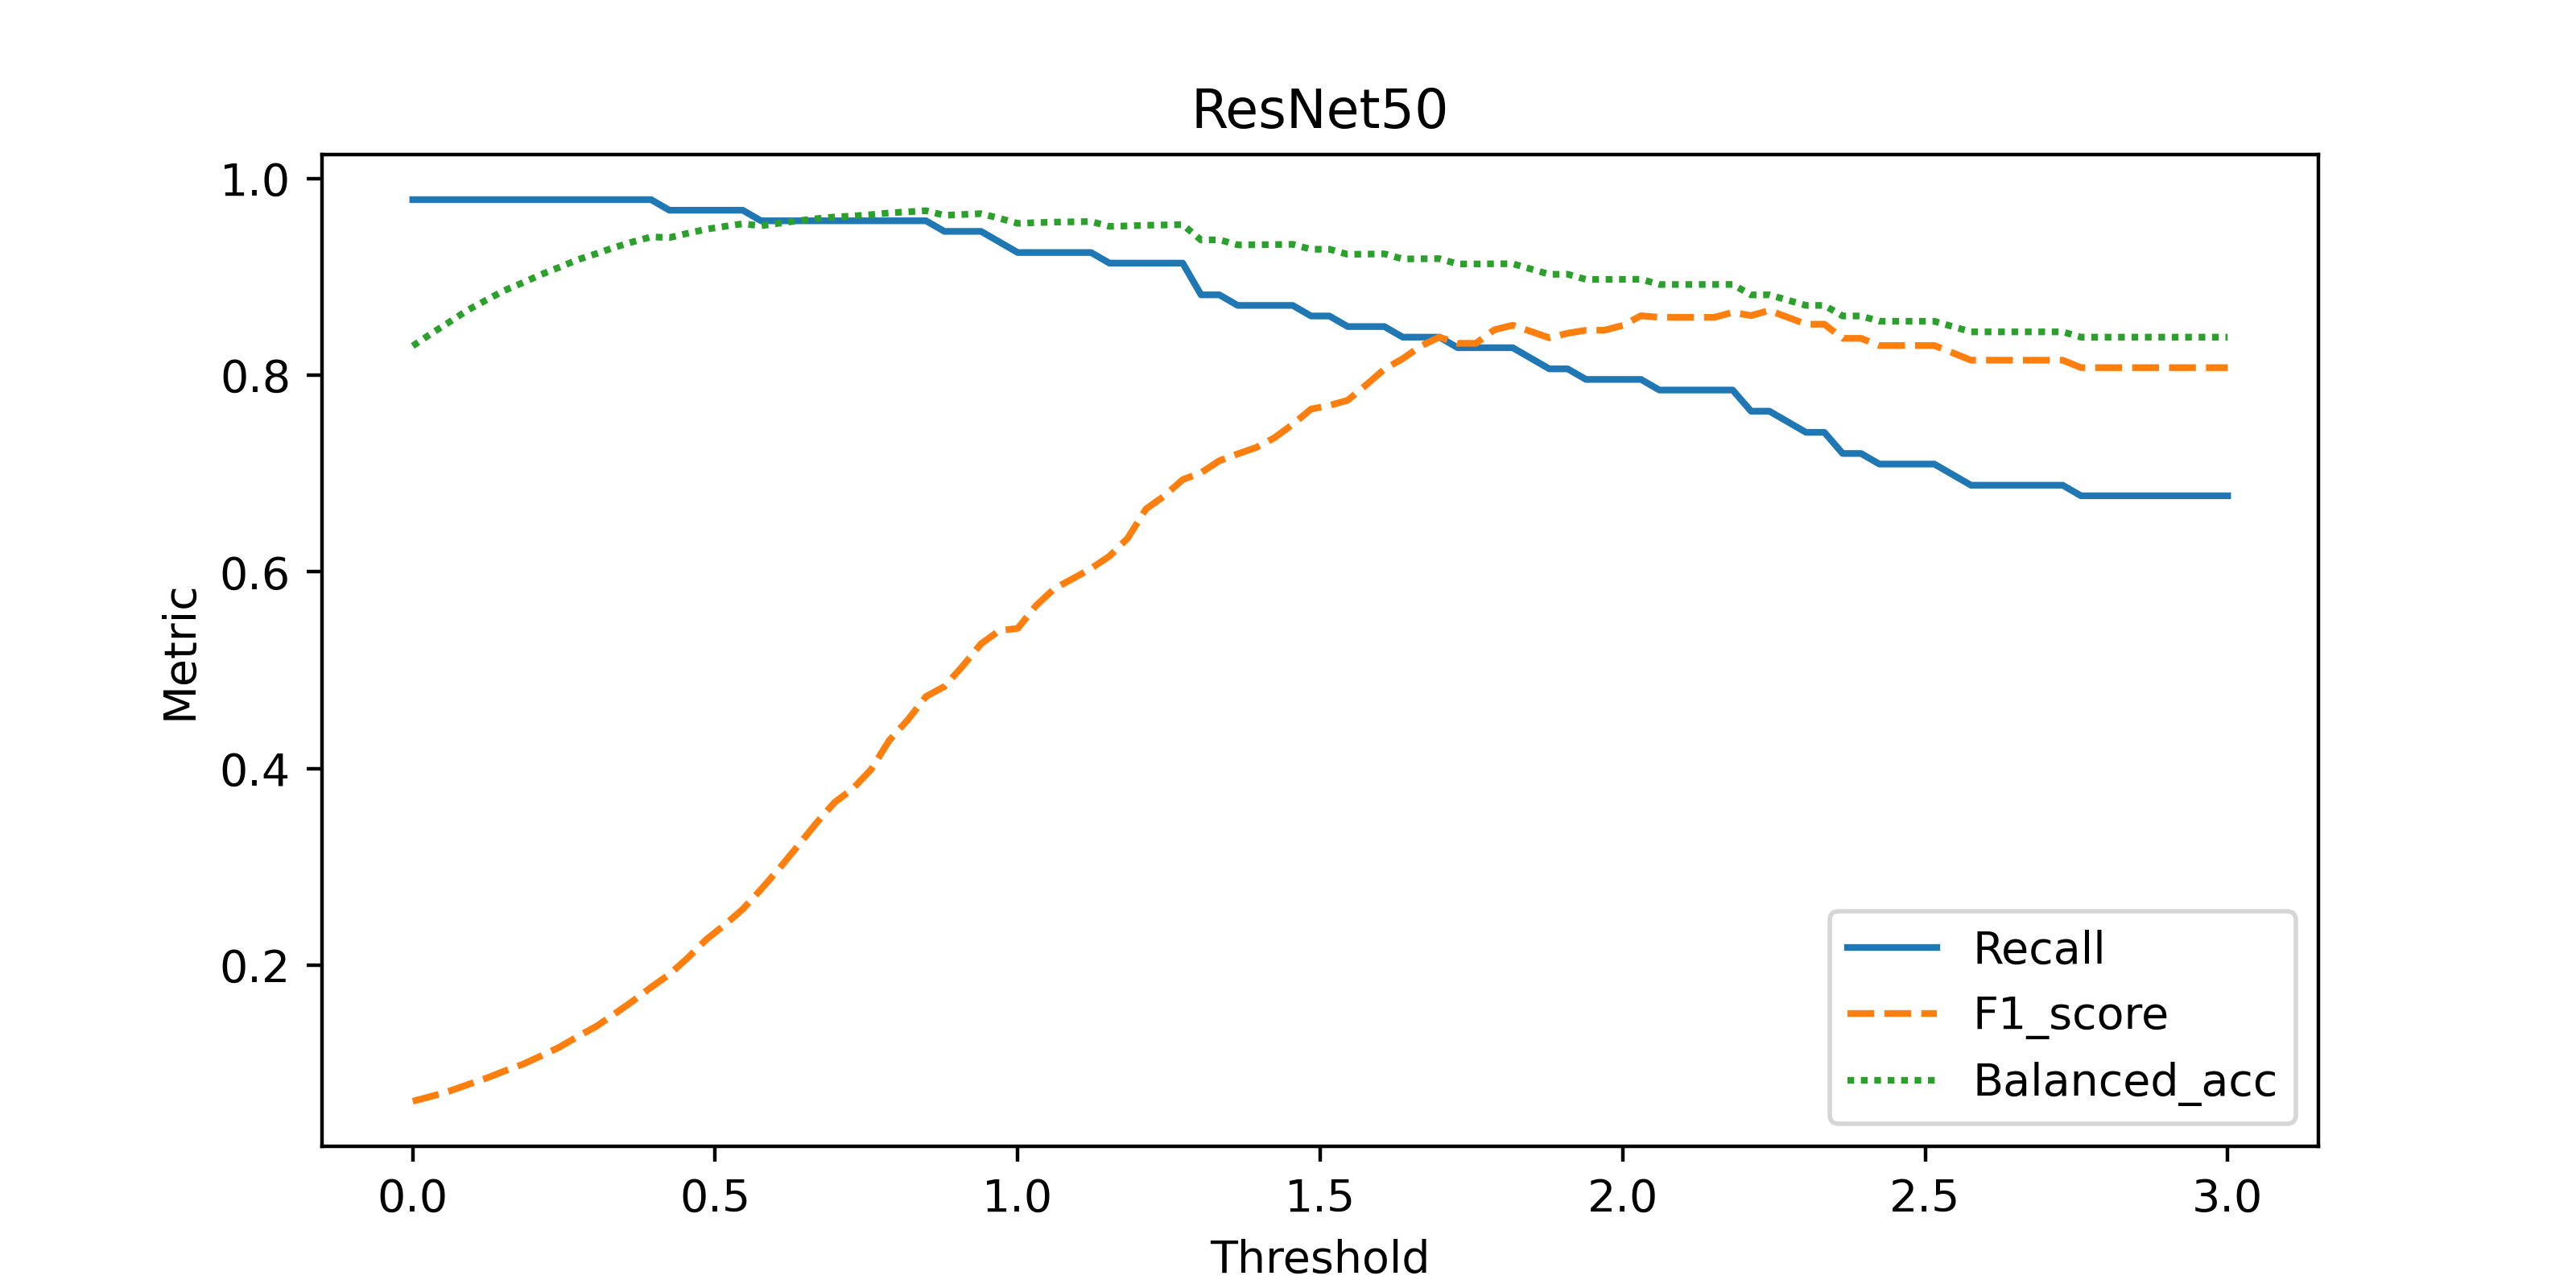
\includegraphics[width=\columnwidth]{./results/comparison/ResNet50_threshold.png}
            \end{figure}
        \end{column}
        \begin{column}{0.45\textwidth}
            \begin{figure}
                \centering
                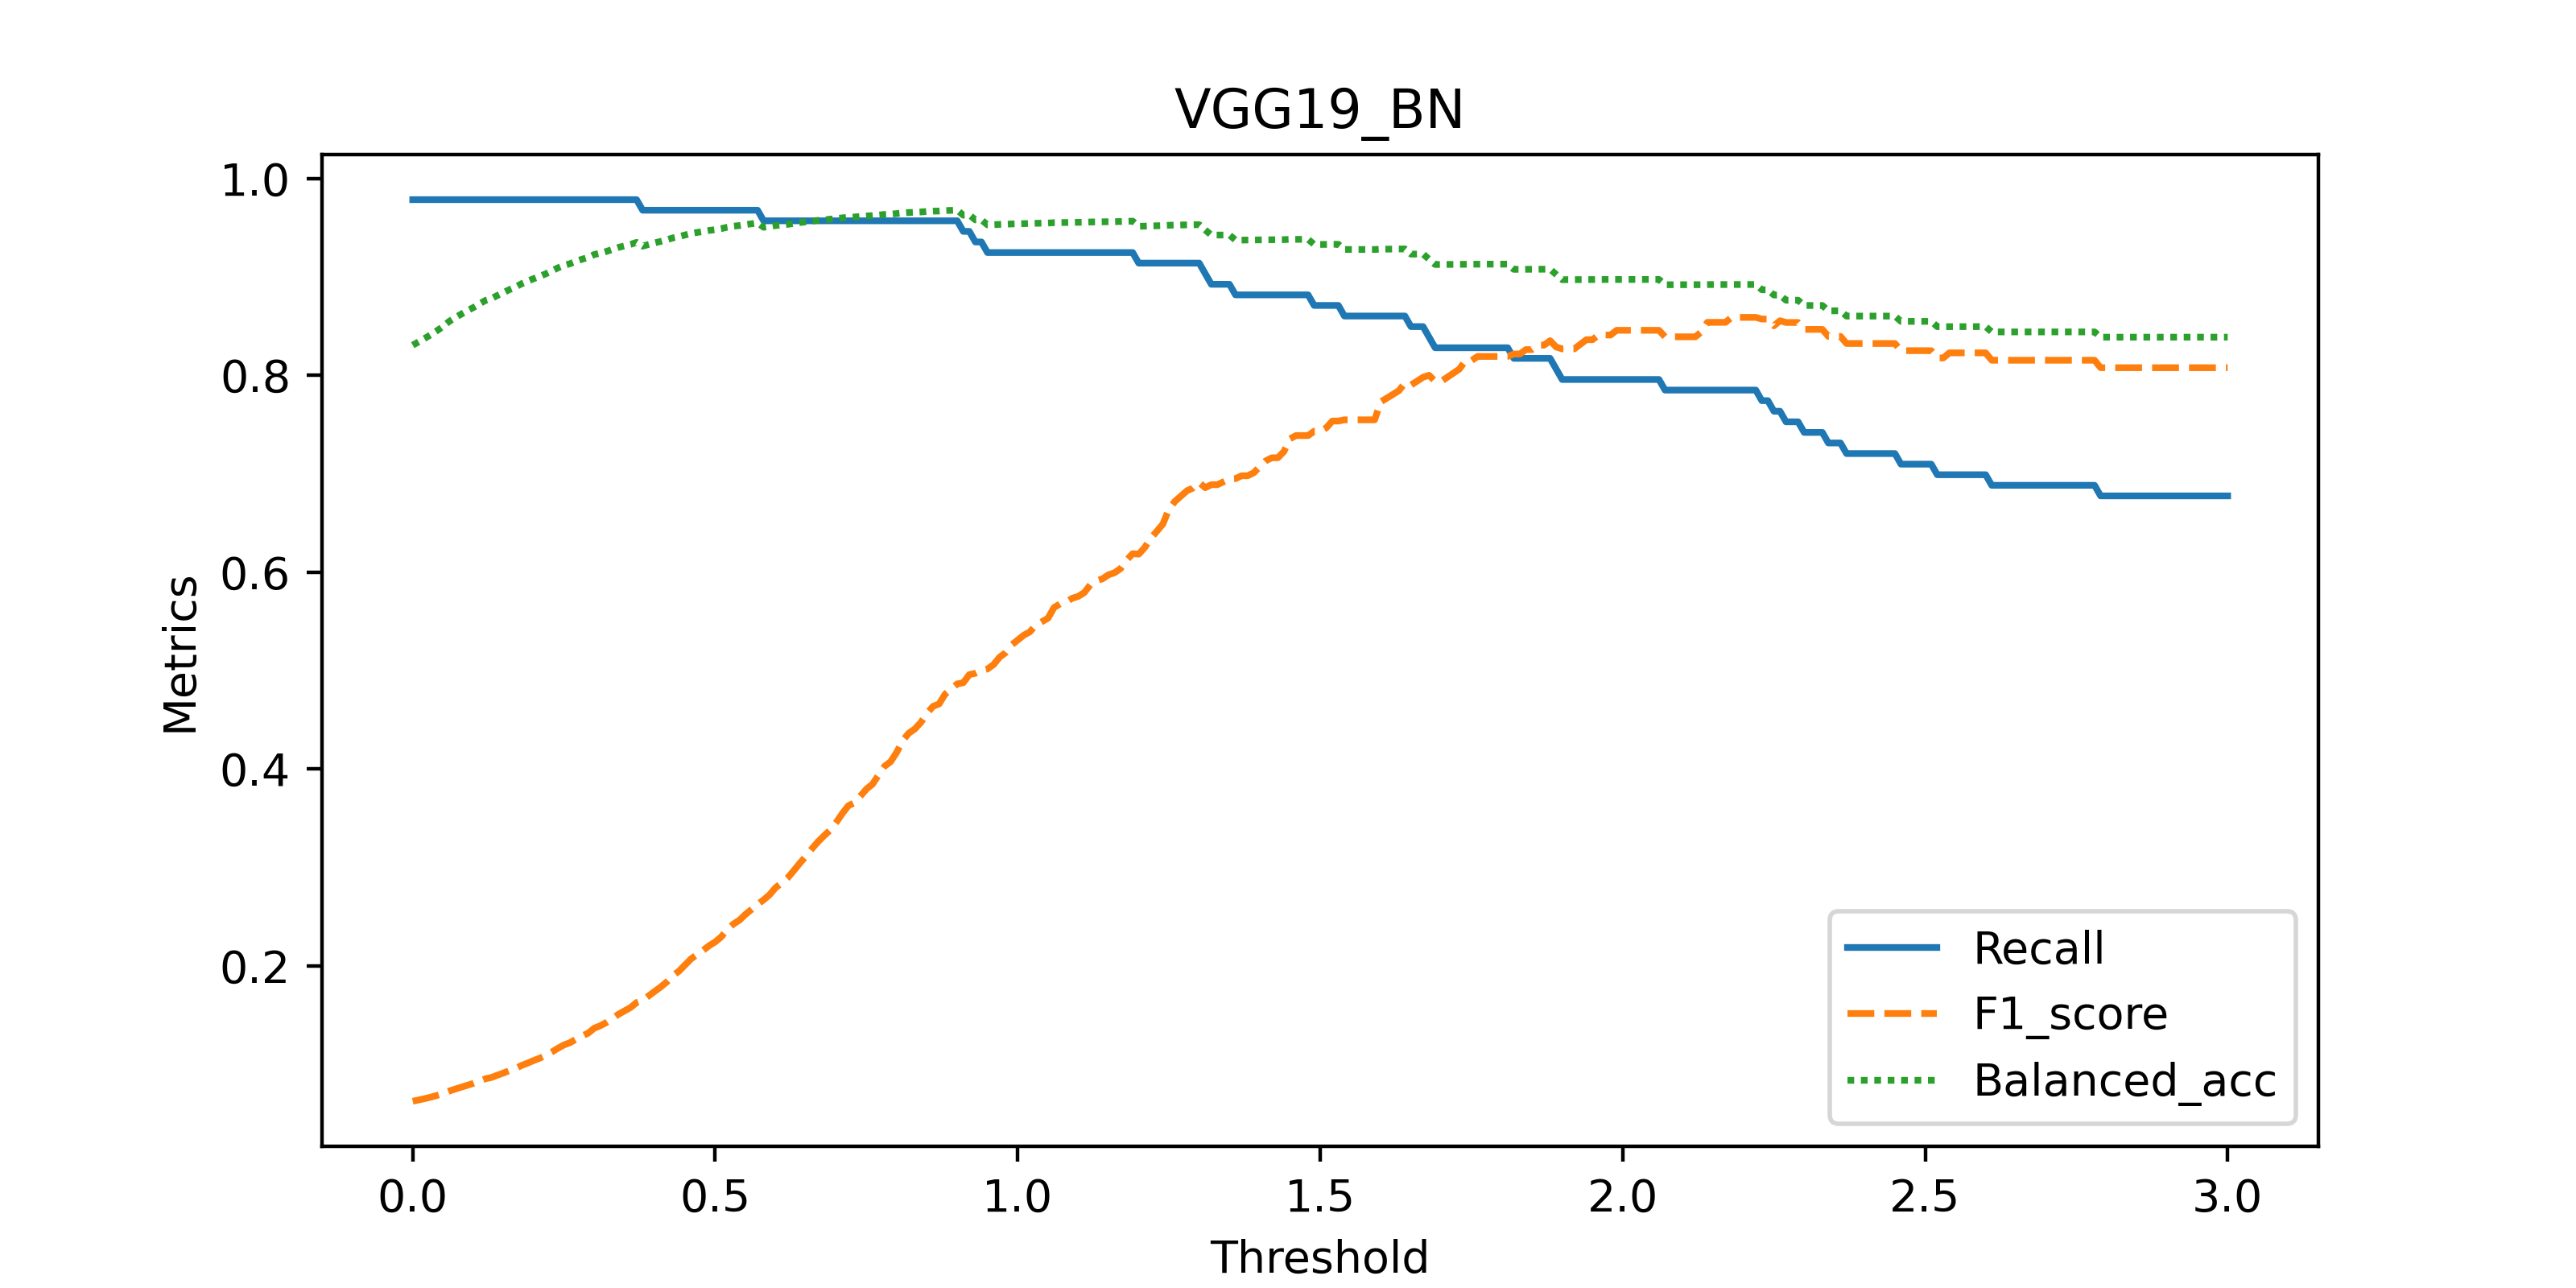
\includegraphics[width=\columnwidth]{./results/comparison/VGG19_BN_threshold.png}
                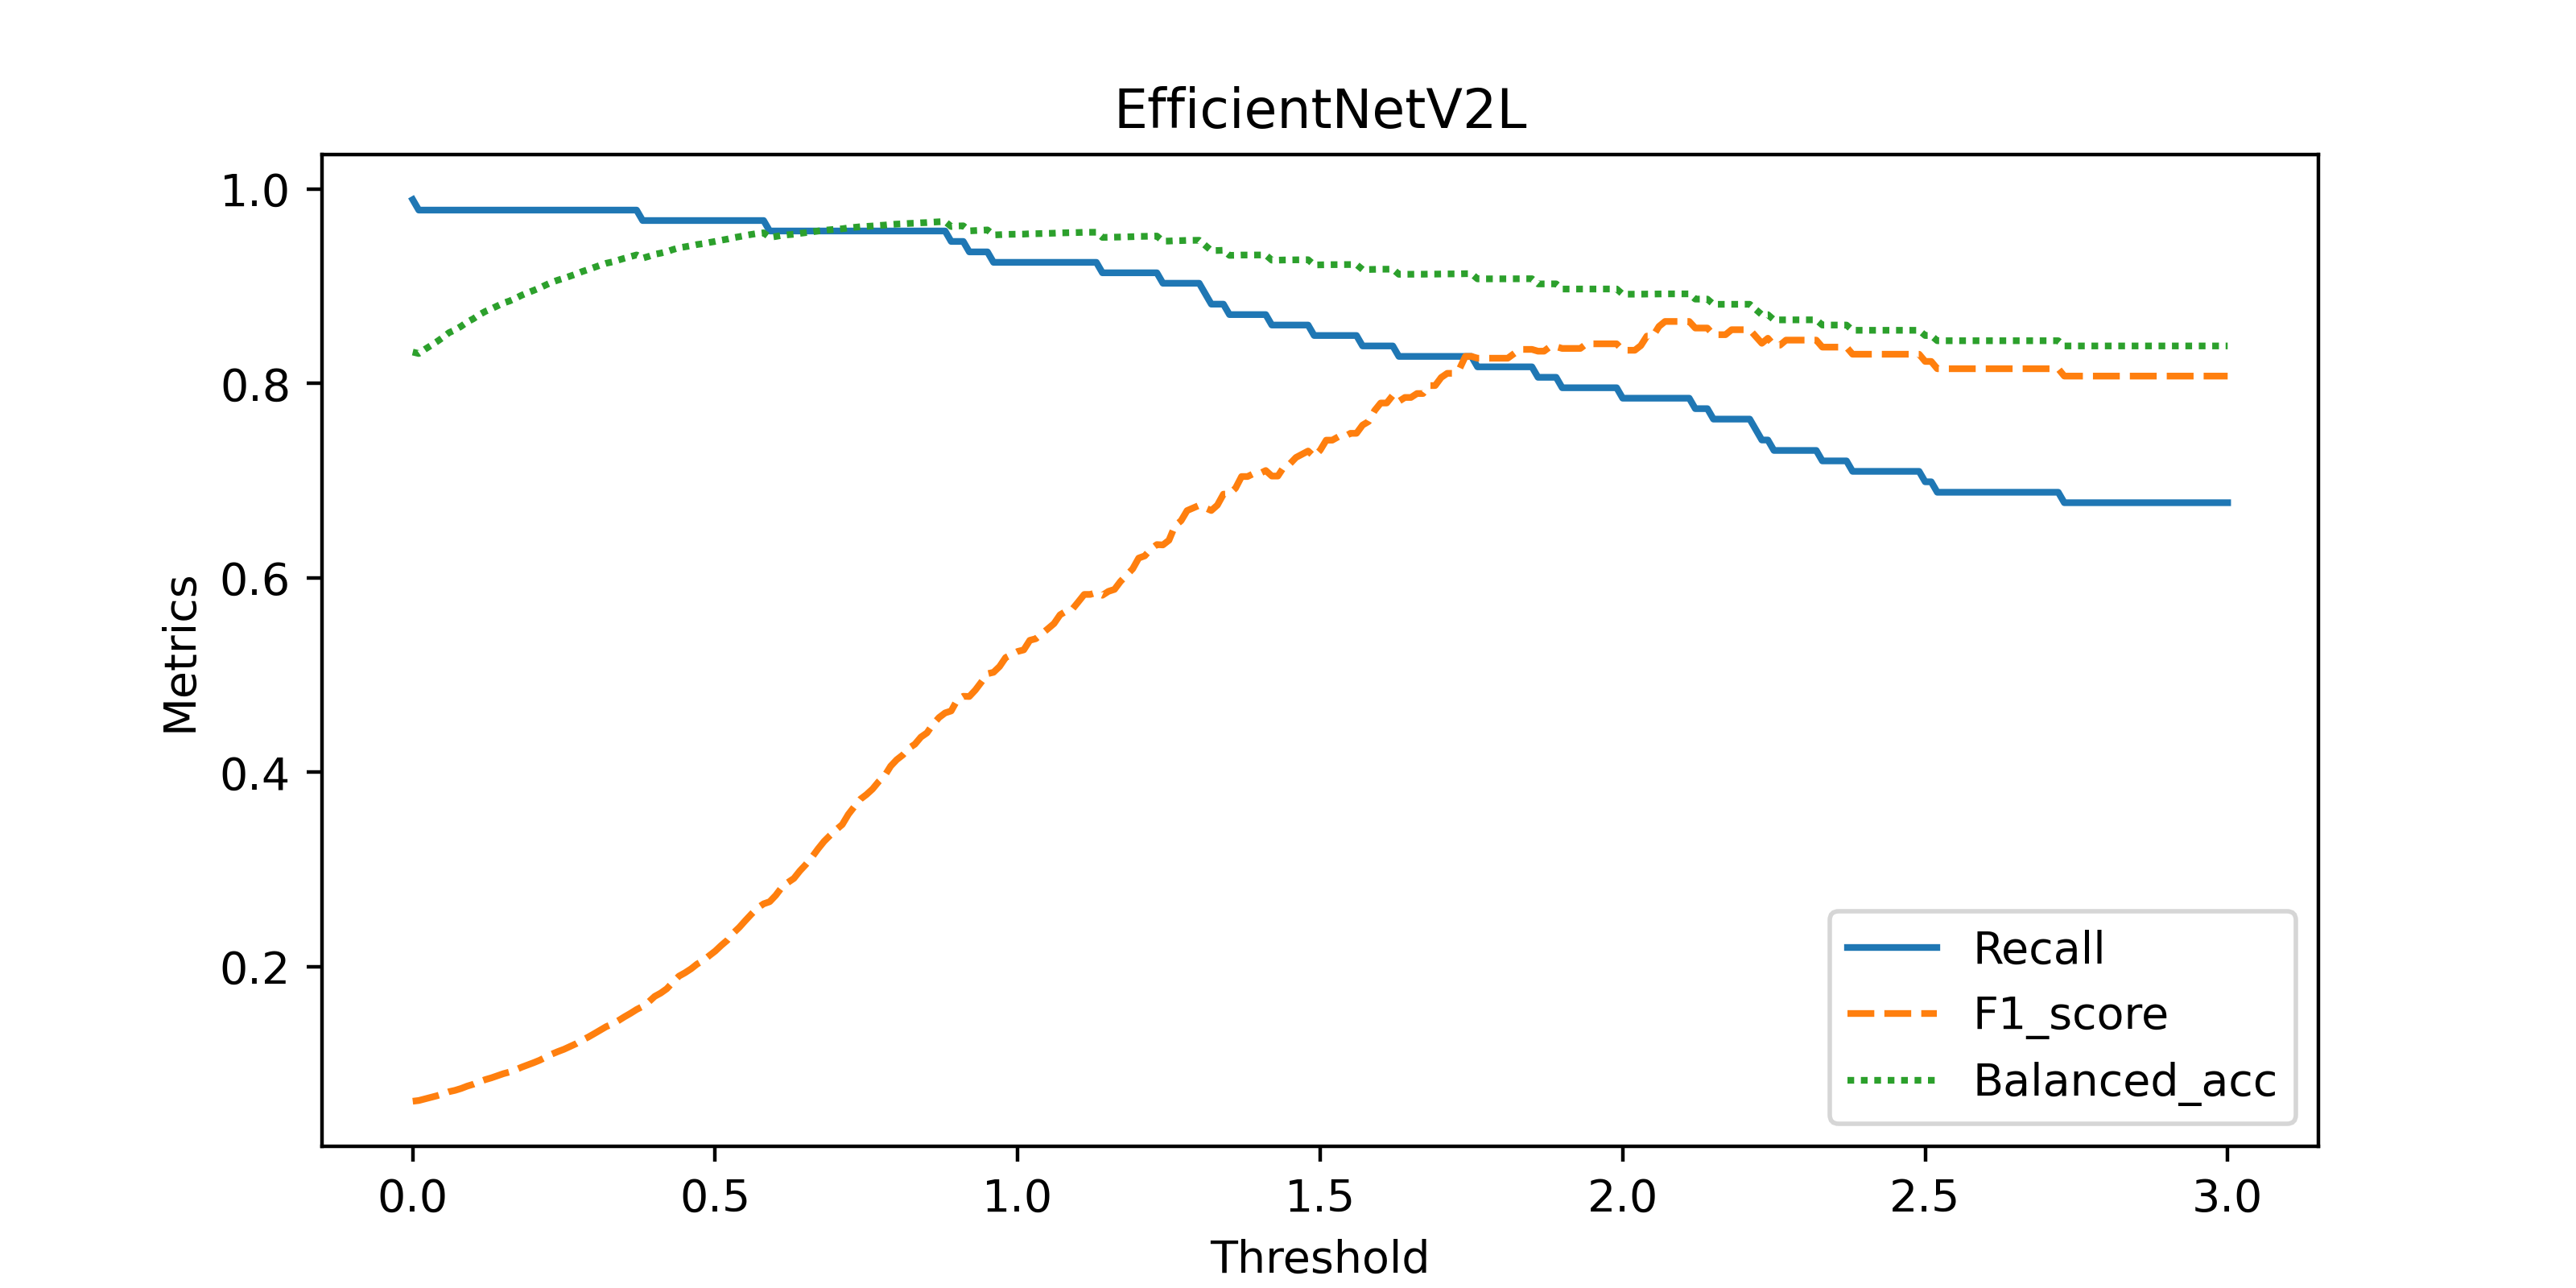
\includegraphics[width=\columnwidth]{./results/comparison/EfficientNetV2L_threshold.png}
            \end{figure}
        \end{column}
    \end{columns}
\end{frame}

\begin{frame}{Detected anomalies}
    \begin{figure}
        \centering
        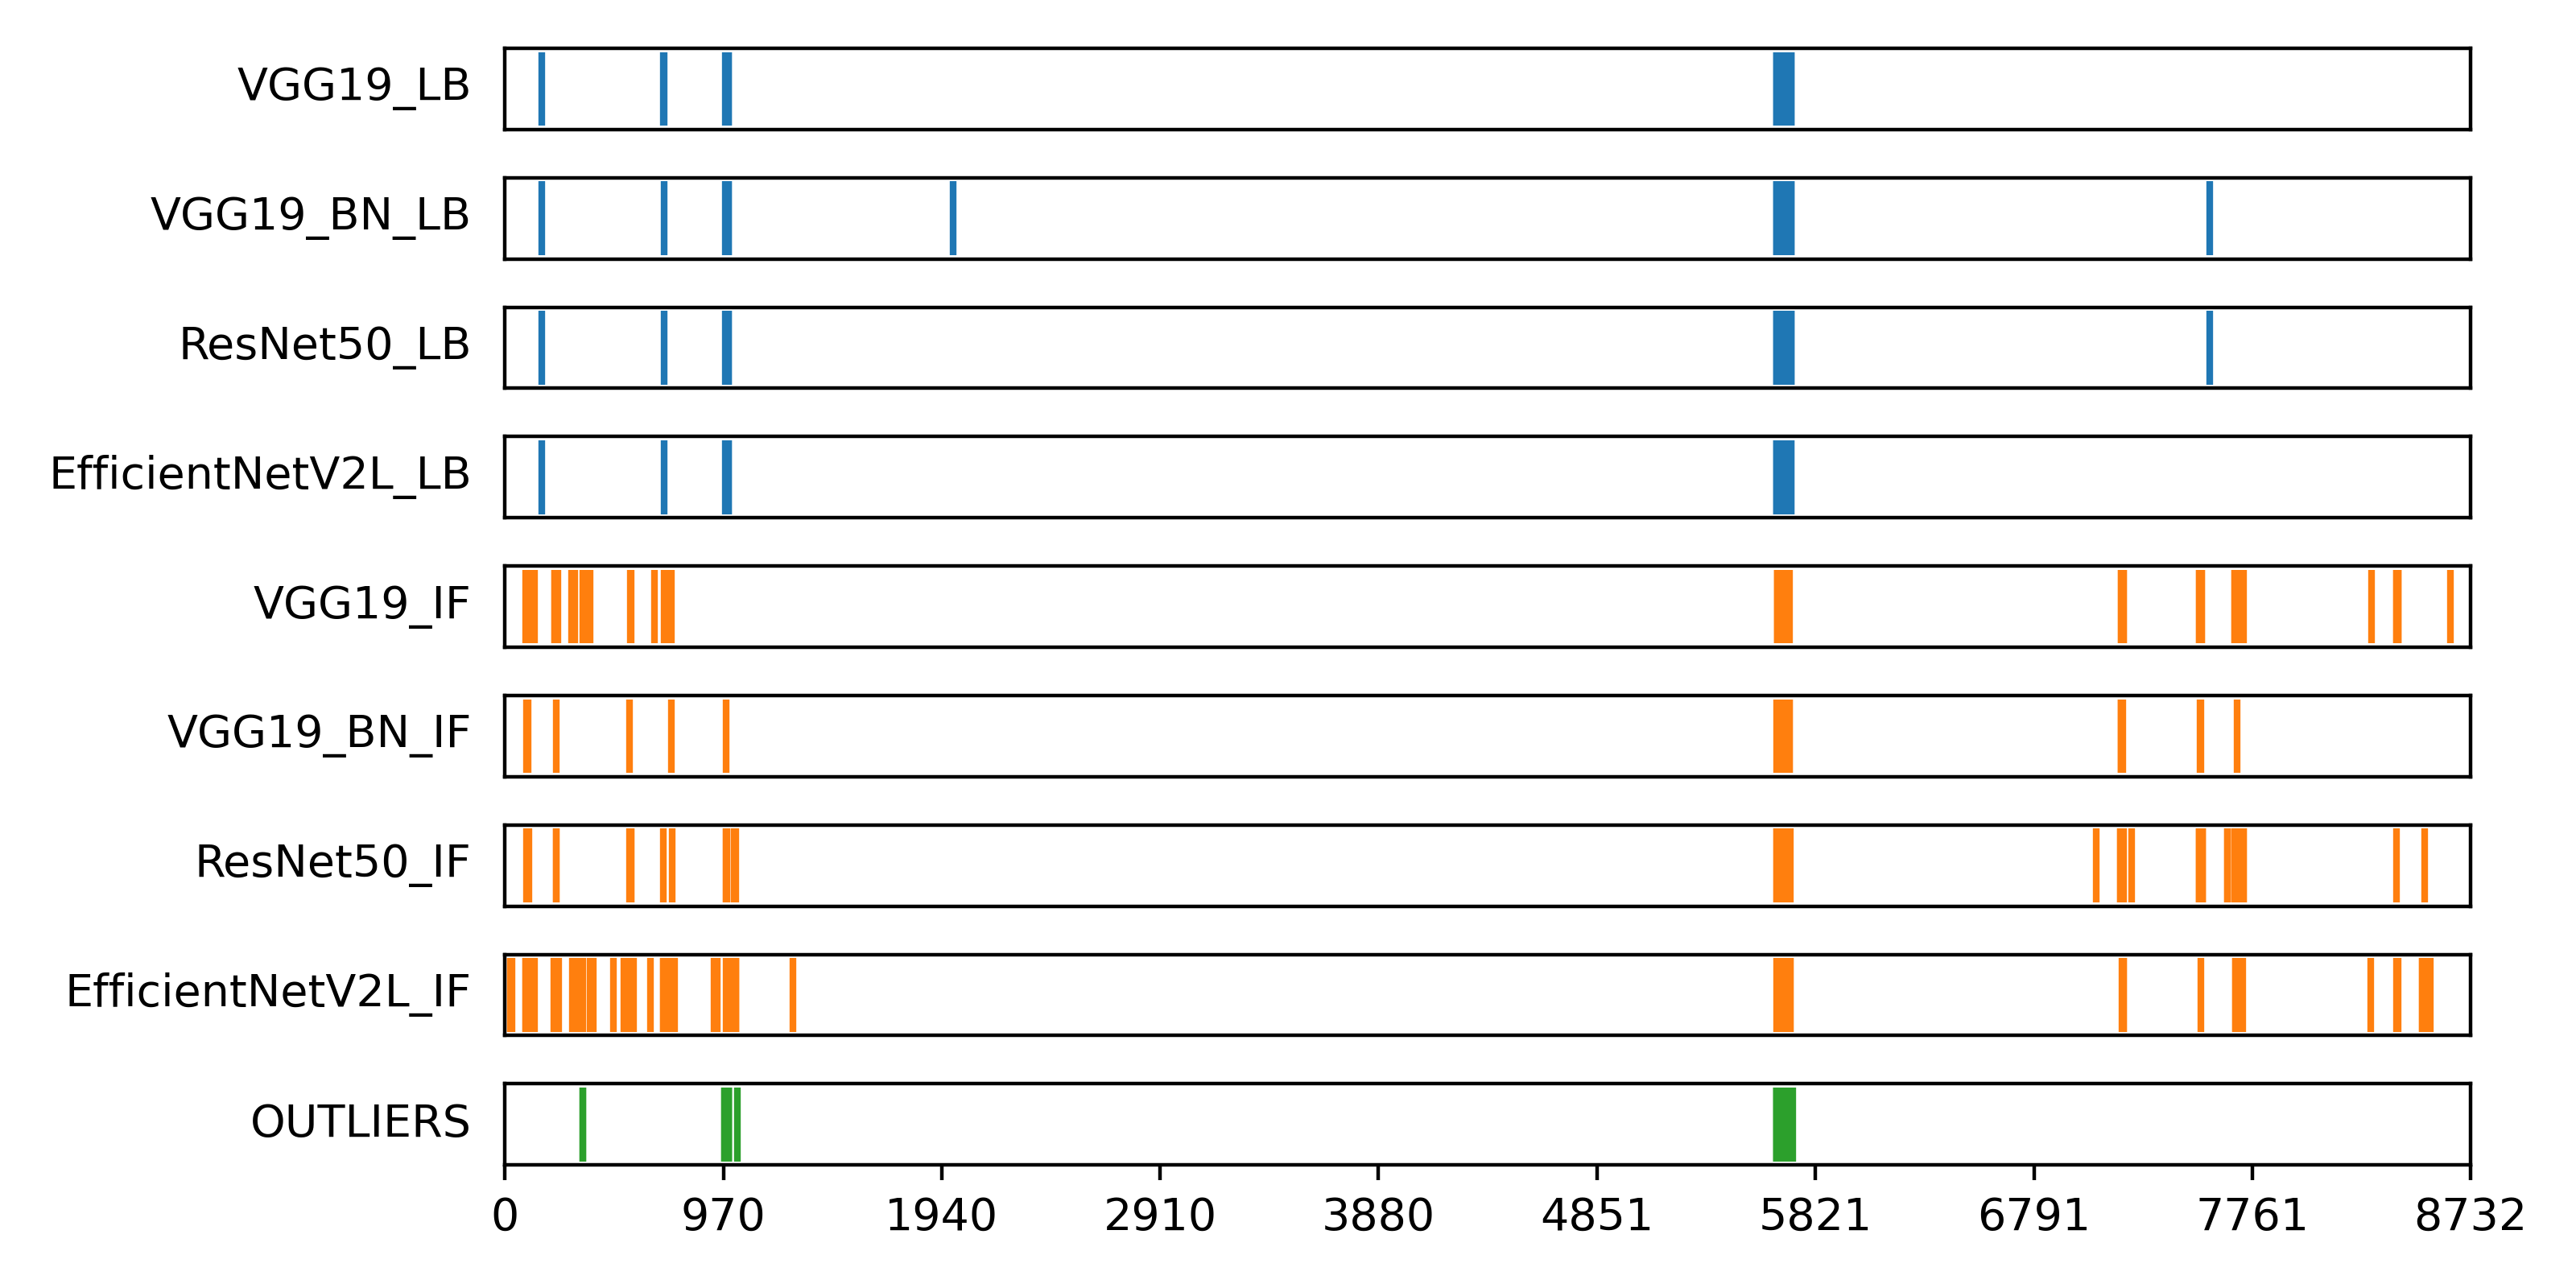
\includegraphics[width=0.9\textwidth]{./results/comparison/outlier_comparison.png}
    \end{figure}
\end{frame}

\begin{frame}{Anomaly clusters and false positives}
    \begin{columns}
        \begin{column}{0.45\textwidth}
            \begin{figure}
                \centering
                \includegraphics[height=0.2\textheight]{./data/sd1_sample/grass/img_00345.jpg}
                \includegraphics[height=0.2\textheight]{./data/sd1_sample/grass/img_00975.jpg}
                \includegraphics[height=0.2\textheight]{./data/sd1_sample/grass/img_05666.jpg}
                \includegraphics[height=0.2\textheight]{./data/sd1_sample/double_rail/img_05677.jpg}
            \end{figure}
        \end{column}
        \begin{column}{0.45\textwidth}
            \begin{figure}
                \centering
                \includegraphics[height=0.2\textheight]{./data/sd1_sample/normal/img_00163.jpg}
                \includegraphics[height=0.2\textheight]{./data/sd1_sample/normal/img_00707.jpg}
                \includegraphics[height=0.2\textheight]{./data/sd1_sample/normal/img_07573.jpg}
            \end{figure}
        \end{column}
    \end{columns}
\end{frame}

\section{Conclusion}
\begin{frame}{Conclusion and outlook}
    \begin{columns}[t]
        \begin{column}{0.45\textwidth}
            Conclusion
            \begin{itemize}
                \item Sample video processed with four different encoders
                \item Applied two outlier detection methods
                \item Major outliers identified
                \item Behavior of NN is visualized using PCA and t-SNE
            \end{itemize}
        \end{column}
        \begin{column}{0.45\textwidth}
            Next steps
            \begin{itemize}
                \item Image processing (histogram equalization)
                \item Further models (NN, anomaly detection)
                \item Model refinement, hyperparameter optimization
                \item Further loss definitions
                \item Segmentation of the image to limit action zone
            \end{itemize}
        \end{column}
    \end{columns}
\end{frame}

\begin{frame}
    \thispagestyle{empty}
    \centering \Large
    Thank you very much for your kind attention!
\end{frame}

\end{document}